%%%%%%%%%%%%%%%%%%%%%%%%%%%%%%%%%%%%%%%%%%%%%%%%%%%%%%%%%%%%%%%%%%%%%%%%%%%%%%%%
%\documentclass[12pt,papel,twoside]{ibtesis}
\documentclass{ibtesis}

% \documentclass[12pt,papel,singlespace,oneside]{ibtesis}
% \documentclass[12pt,papel,preprint,singlespace,oneside]{ibtesis}

%%%%%%%%%%%%%%%%%%%%% Paquetes extra %%%%%%%%%%%%%%%%%%%%%%%%%%%%%%%%%%%%%%%%%%%
% Por conveniencia: aqu\'{\i} puede cargar todos los paquetes y definir los comandos 
% que necesite
\usepackage{ibextra}
\usepackage[utf8]{inputenc}
\usepackage{subcaption}  % Enable figure captions or figure notes
\usepackage{float}
\usepackage{nicefrac}
\usepackage{mathtools}
\usepackage{textcomp}

\usepackage{amsfonts}

\newcommand{\done}{\item[\checkmark]}
%%%%%%%%%%%%%%%%%%%%%%%%%%%%%%%%%%%%%%%%%%%%%%%%%%%%%%%%%%%%%%%%%%%%%%%%%%%%%%%%
%%%%%%%%%%%%%%%%%%%%% Informacion sobre la tesis %%%%%%%%%%%%%%%%%%%%%%%%%%%%%%%
\title{Merge reports}
\author{Evelyn~G.~Coronel}
\director{Dra.~Silvia Mollerach}
%\codirector{Dr.~J.~Otro m\'{a}s}b
\carrera{Tesis de Maestría en Ciencias F\'{\i}sicas}
\grado{Maestrando}
\laboratorio{Partículas y Campos -- Centro At\'{o}mico Bariloche}
\jurado{Dr.~Diego~Harari (Instituto Balseiro)}

\palabrasclave{Rayos Cósmicos, Análisis de datos, Instituto Balseiro}
%\keywords{Cosmic Rays, Data Analysis, Balseiro Institute}
\neembaeguasu{Mba'e michĩ yvágagui ouva, Mbo'ehaoguasu Balseiro}
% Si queremos poner la fecha manualmente:
% \date{Diciembre de 2099}

%%%%%%%%%%%%%%%%%%%%%%%%%%%%%%%%%%%%%%%%%%%%%%%%%%%%%%%%%%%%%%%%%%%%%%%%%%%%%%%%
\titlepagefalse 
%%%%%%%%%%%%%%%%%%%%%%%%%%%%%%%%%%%%%%%%%%%%%%%%%%%%%%%%%%%%%%%%%%%%%%%%%%%%%%%%


%\setcounter{tocdepth}{4}
%\setcounter{secnumdepth}{4}
\begin{document}

\chapter{report 1 13 04 2020}

\graphicspath{{report_1_13_04_2020/}}

\section{Dudas sobre los pesos}

¿Por qué verifico esto? Los pesos son importantes para el cálculo de anisotropías, porque las anisotropías son pequeñas y eliminar todo factor espúreo es importante.

¿Por qué me trabé tanto? Cuando uso sólo 24 bines, los números entre el paper del 2018 y los que obtengo con mi código son parecidos. En cambio cuando otro bineado, como 360 bines, con el mismo código, hay una diferencia entre lo que se obtiene en el paper mencionado y el mi tesis.

¿Por qué creo que está pasando esto? Si el código funciona para 24 bines, como se muestra en la Fig.\,\ref{fig:all_24}, y cuando sólo cambio la cantidad de bines, como en las Fig.\,\ref{fig:sid_360} y \ref{fig:anti_360}, se ve que sigue la misma tendencia pero no los mismos números. Yo lo que yo creo es que tiene que ver con la precisión del cálculo. Para calcular cada punto, se realiza una división entre dos números, i.e. 
\begin{equation}
	\Delta N = \frac{\text{Los hexágonos integrados en un bin}}{\text{Todos los hexágonos integrados para cada bin}}
\end{equation}


\begin{figure}[H]
	\centering
	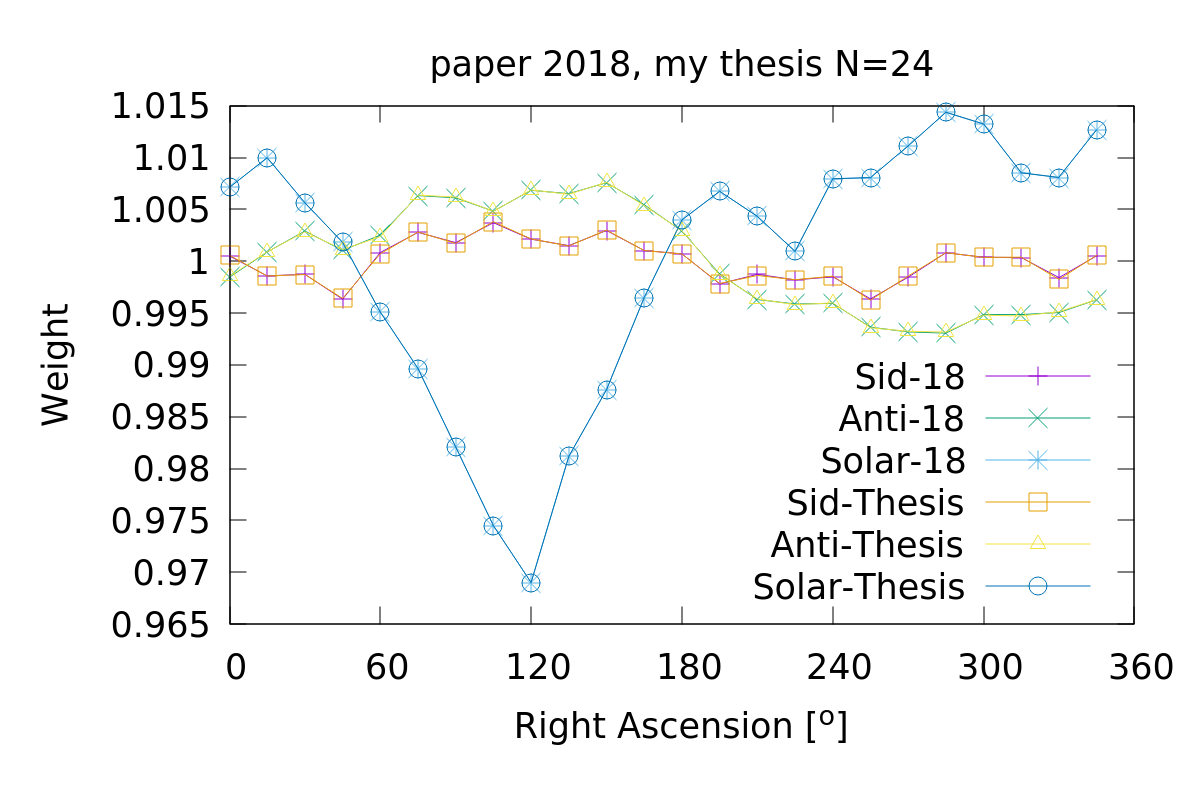
\includegraphics[width=0.45\textwidth]{solar_anti_sid_my_and_paper_in_24.png}
	\caption{Usando 24 bines para las frecuencias sidérea, anti-sidérea y solar, se compara el paper del 2018 con lo que obtengo en la tesis.}
	\label{fig:all_24}
\end{figure}


En el caso de $N=24$, son dos números grandes, por lo tanto solo importan los primeros número a izquierda, pero para  $N=360$ es como menor. Durante la ejecución del programa, para cada valor de utc, se calcula a que bin corresponde esa entrada; verifiqué que el programa del paper y mío fuera iguales a cada paso, y constaté que no había diferencias.

Debido a esto, mi hipótesis es la diferencia entre ambos códigos es por la suma de hexágonos. Lo que me causa ruido de esto es que la diferencia entre los puntos del paper y de mi código, para la frecuencia sidérea,  no es ruido centrado en cero como esperaría que fuera si es un error en la precisión, como se muestra en la Fig.\ref{fig:error_360_sid}, lo que me hace dudar de mi hipótesis. En cambio para la frecuencia anti-sidérea, como se ve en la Fig.\ref{fig:error_360_anti}, el error no tiene ninguna modulación.

\begin{figure}[H]
	\centering
	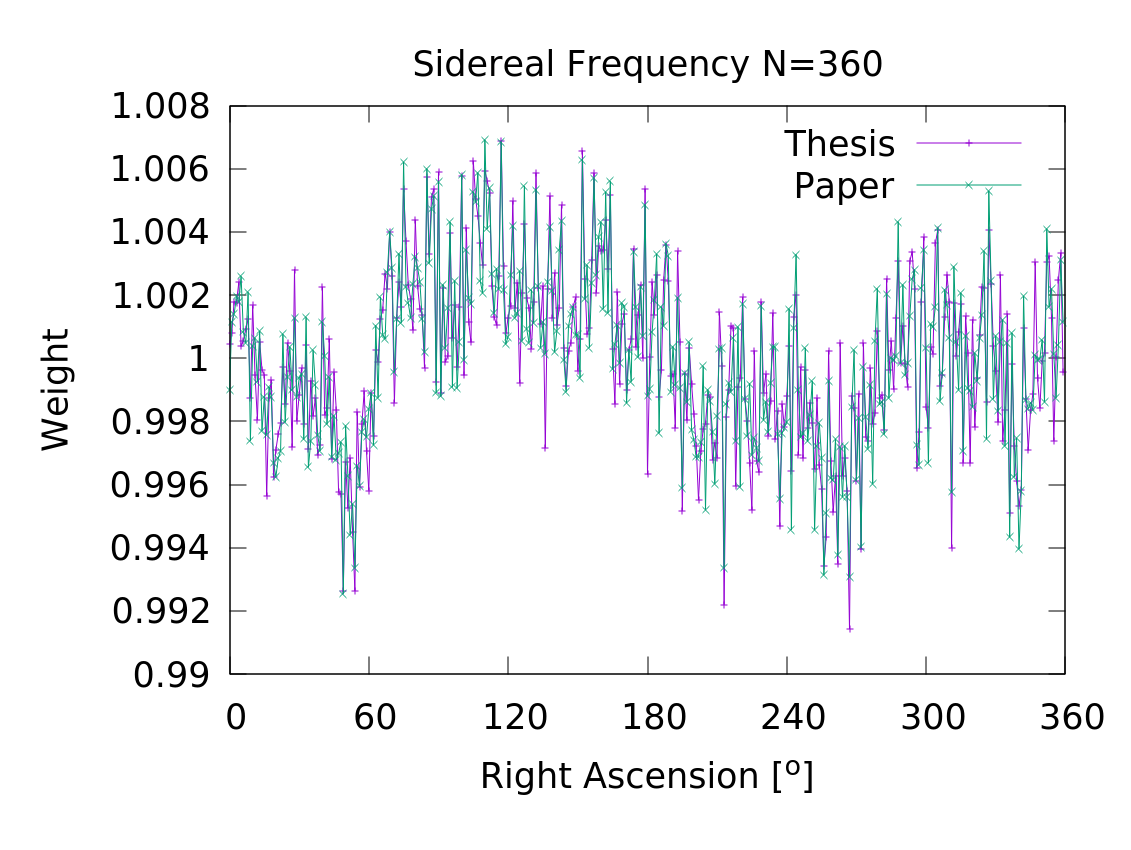
\includegraphics[width=0.45\textwidth]{sidereal_my_and_paper_in_360.png}
	\caption{Usando 360 bines para la frecuencia sidérea.}
	\label{fig:sid_360}
\end{figure}


\begin{figure}[H]
	\centering
	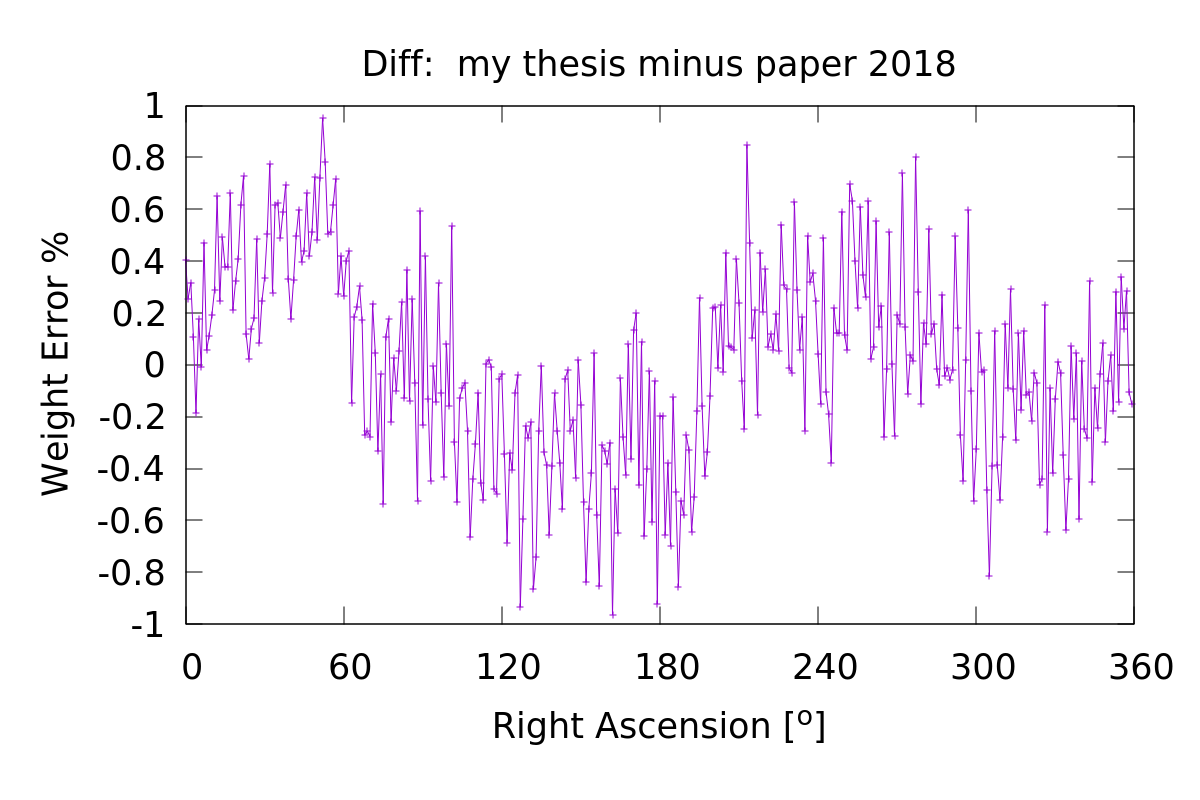
\includegraphics[width=0.45\textwidth]{sidereal_my_and_paper_in_360_error.png}
	\caption{Usando los valores del paper como referencia, calculé el error porcentual con lo que yo obtengo para la frecuencia sidérea.}
	\label{fig:error_360_sid}
\end{figure}



\begin{figure}[H]
	\centering
	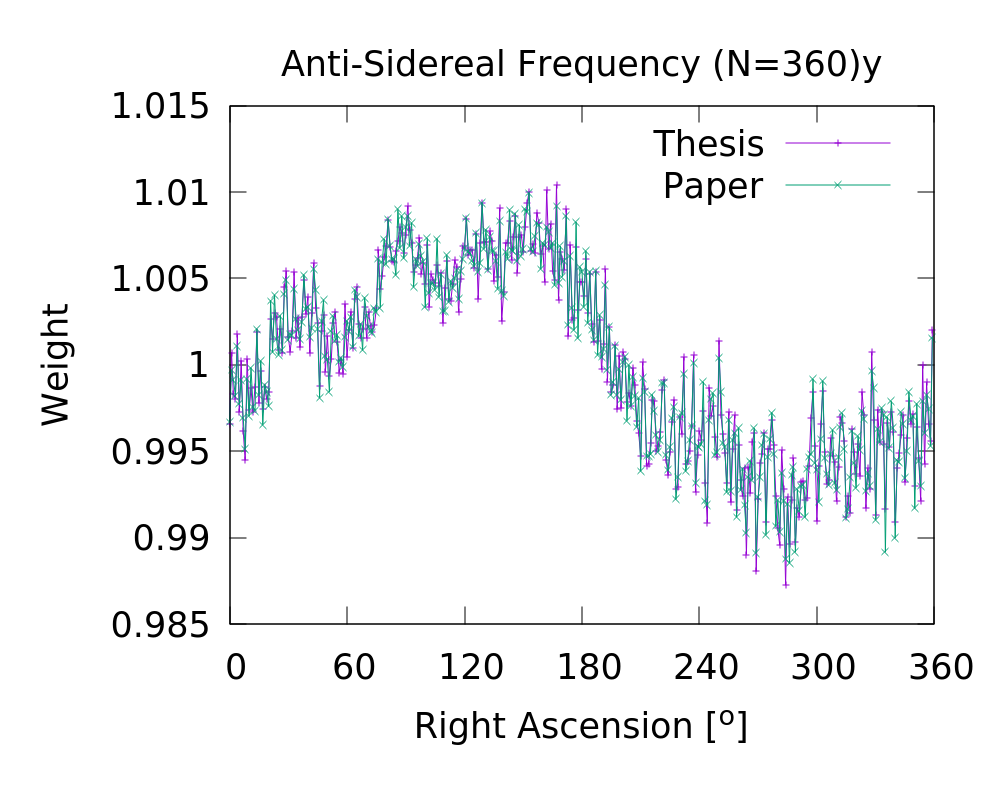
\includegraphics[width=0.45\textwidth]{anti_my_and_paper_in_360.png}
	\caption{Usando 360 bines}
	\label{fig:anti_360}
\end{figure}


\begin{figure}[H]
	\centering
	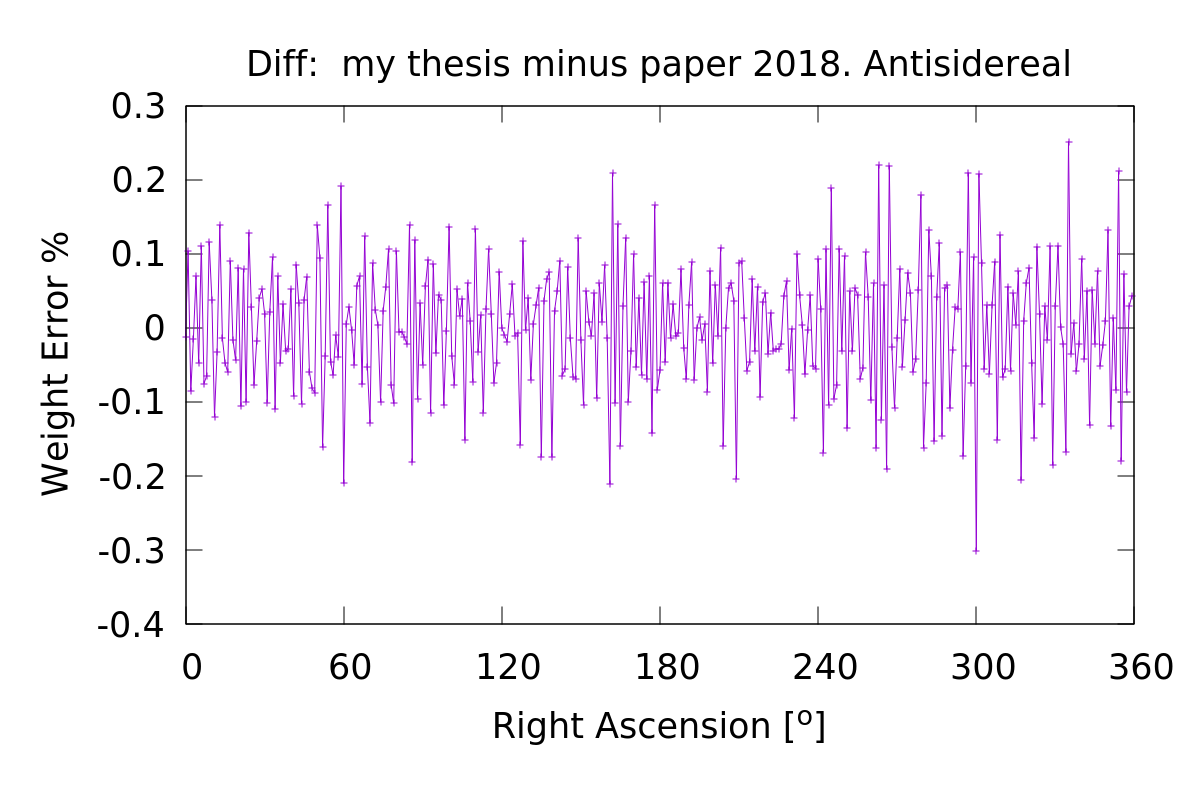
\includegraphics[width=0.45\textwidth]{anti_my_and_paper_in_360_error.png}
	\caption{Usando los valores del paper como referencia, calculé el error porcentual de la frecuencia anti-sidérea.}
	\label{fig:error_360_anti}
\end{figure}



\section{Duda sobre los algoritmos}

Contexto: Yo quiero hacer el análisis de los pesos de los hexágonos para distintas frecuencias, por lo que esperaría que para cada frecuencia a analizar se utilice el mismo algoritmo para todos.

Mi duda: En el código del paper 18, el algoritmo hace distinción entre la frecuencia sidérea y las demás. Comparando ambos algoritmos, como se muestra en la Fig.\,\ref{fig:alter_24}, se ve que ambos dan un resultado similar para los pesos de los hexágonos a menos de un desfase de $75^o$ o $5\,$hrs sidéreas. Los gráficos de esta figura se hicieron con el mismo data set.

\begin{figure}[H]
	\centering
	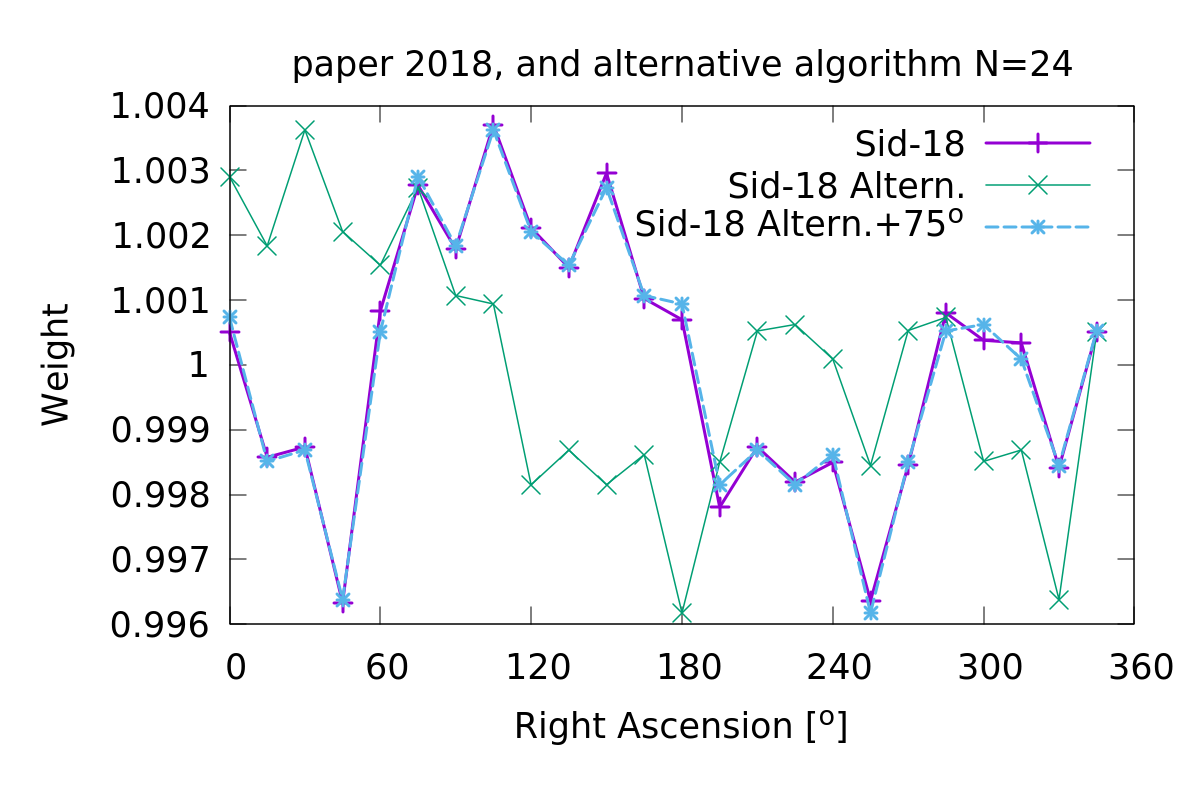
\includegraphics[width=0.45\textwidth]{sidereal_paper_in_24_w_alter.png}
	\caption{Comparando el algoritmo alternativo con el utilizado en el paper 18 con resultados del mismo paper, para 24 bines.}
	\label{fig:alter_24}
\end{figure}


Otra cosa que me resultó curiosa fue que usando $N=360$, tengo problemas con la frecuencia solar, donde aparecen 0 cada 5 min, coincide con el rate de actualización del archivo de weather. Así usando este bineado, aparece ese problema, recomendaría no trabajar con bines de $1^o$ en ascensión recta.
\begin{figure}[H]
	\centering
	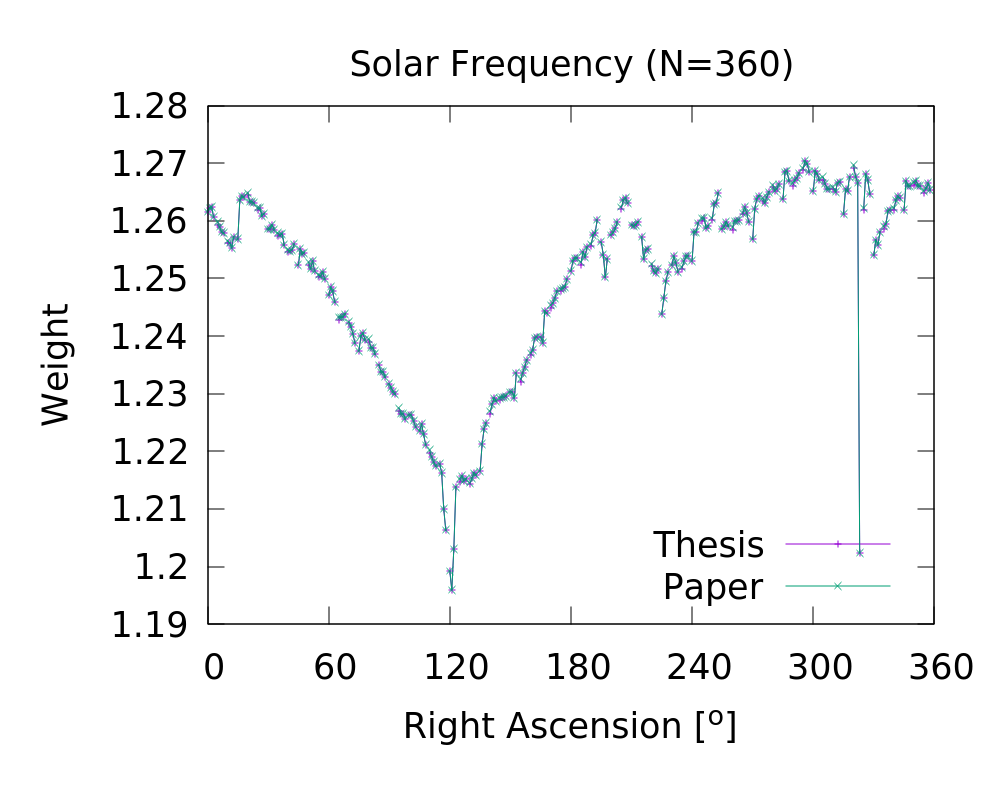
\includegraphics[width=0.45\textwidth]{solar_my_and_paper_in_360_2.png}
	\caption{Usando 360 bines, nótese que la media es distinta a la figura anterior.}
	\label{fig:solar_360}
\end{figure}

\section{Para N=288}

El gráfico que me envió usted, sobre los pesos para estas frecuencias es la Fig.\,\ref{fig:all_288_paper}. La discusión sobre estos resultados en particular es análoga al caso para $N=360$, con la diferencia que no tengo valores de anómalos que se ven para la frecuencia solar, Fig.\,\ref{fig:solar_288}.
\begin{figure}[H]
	\centering
	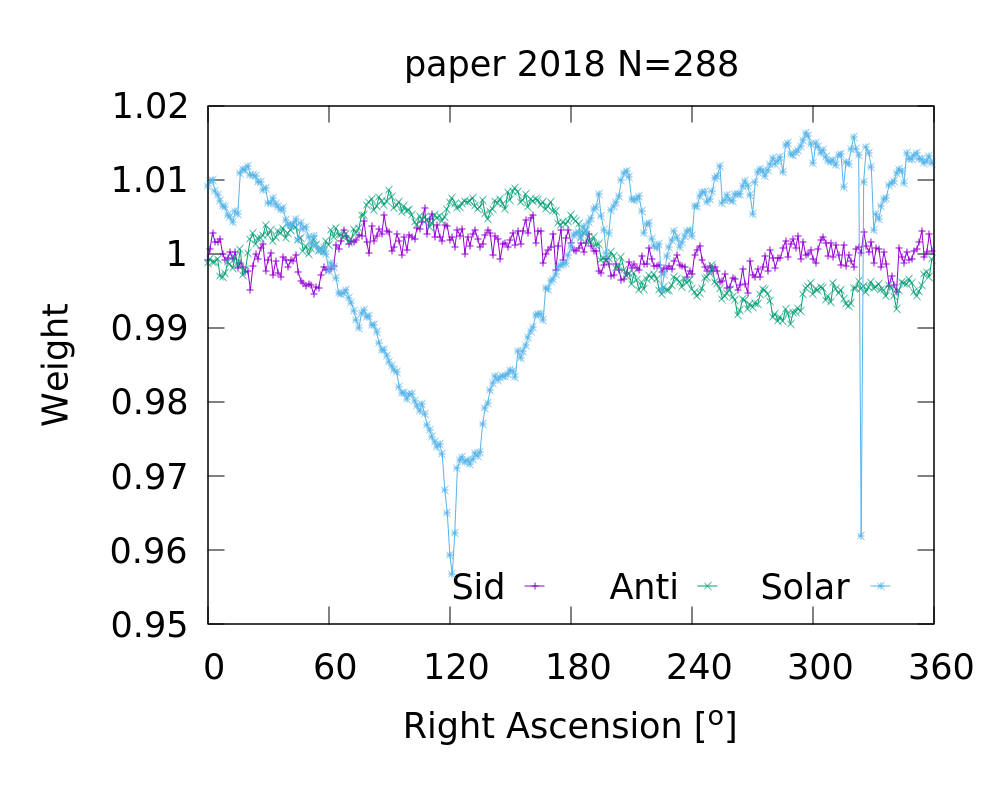
\includegraphics[width=0.45\textwidth]{solar_anti_sid_paper2018_in_288.png}
	\caption{Los pesos para las tres frecuencias tal como se calcula en el paper del 2018.}
	\label{fig:all_288_paper}
\end{figure}



\begin{figure}[H]
	\centering
	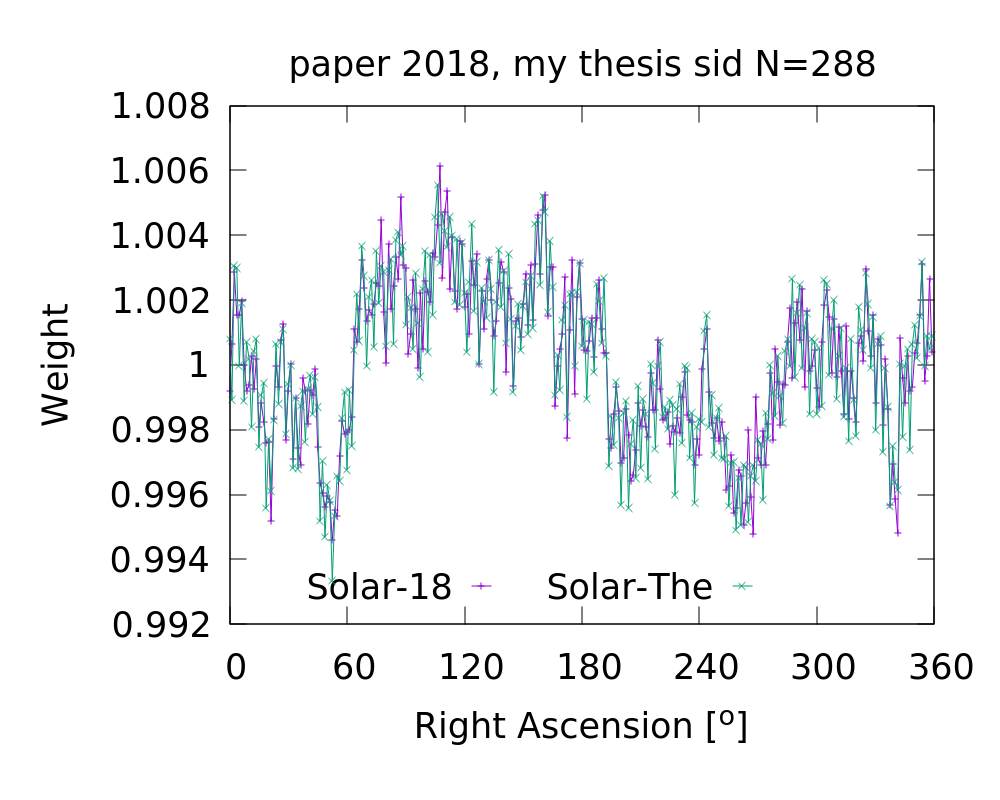
\includegraphics[width=0.45\textwidth]{sidereal_my_and_paper_in_288.png}
	\caption{Comparando los resultados del paper con mi código para la frecuencia sidérea para N=288}
	\label{fig:sidereal_288}
\end{figure}


\begin{figure}[H]
	\centering
	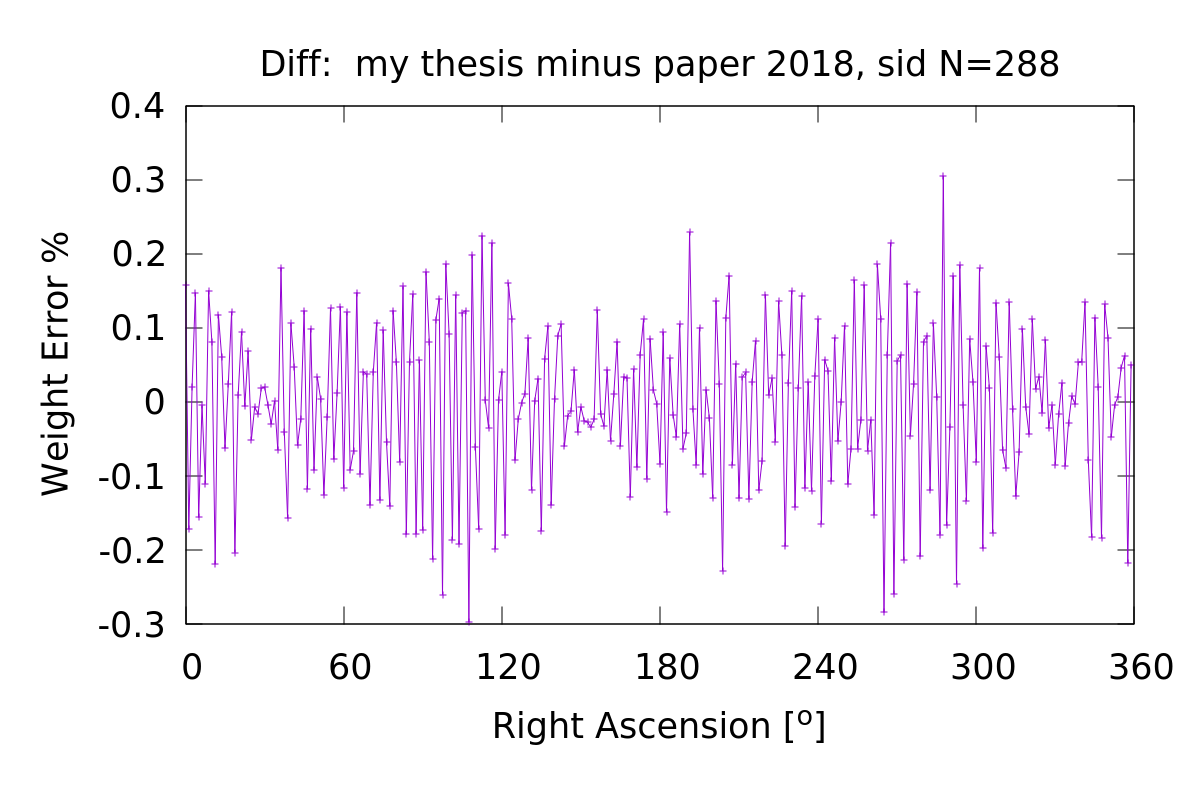
\includegraphics[width=0.45\textwidth]{sidereal_my_and_paper_in_288_error.png}
	\caption{El error porcentual entre lo que obtengo en mi código, usando el paper de referencia.}
	\label{fig:error_288_sidereal}
\end{figure}


Ya en la Fig.\,\ref{fig:sidereal_288}, se ve que la media de los pesos es algo razonable comparándolo con N=360, Fig.\ref{fig:solar_360}. Además que el error porcentual, usando como referencia los resultados del paper del 2018, es pequeña. La misma se muestra en la Fig.\,\ref{fig:error_288_solar}.

\begin{figure}[H]
	\centering
	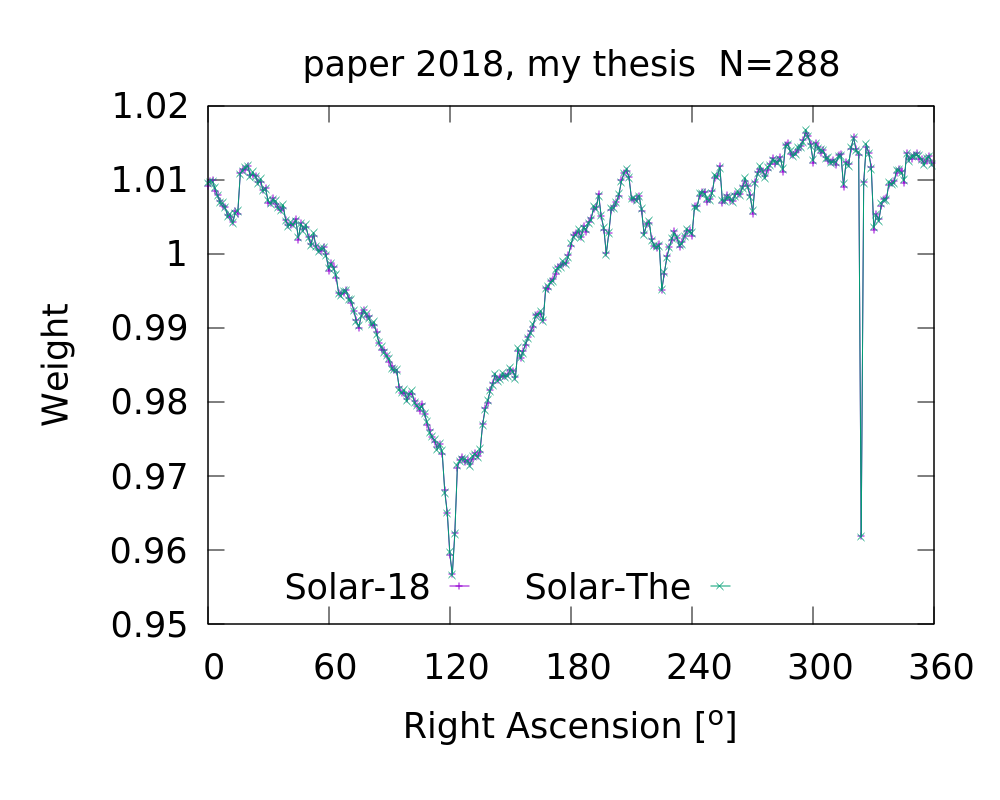
\includegraphics[width=0.45\textwidth]{solar_my_and_paper_2018_in_288.png}
	\caption{Pesos para la frecuencia solar.}
	\label{fig:solar_288}
\end{figure}


\begin{figure}[H]
	\centering
	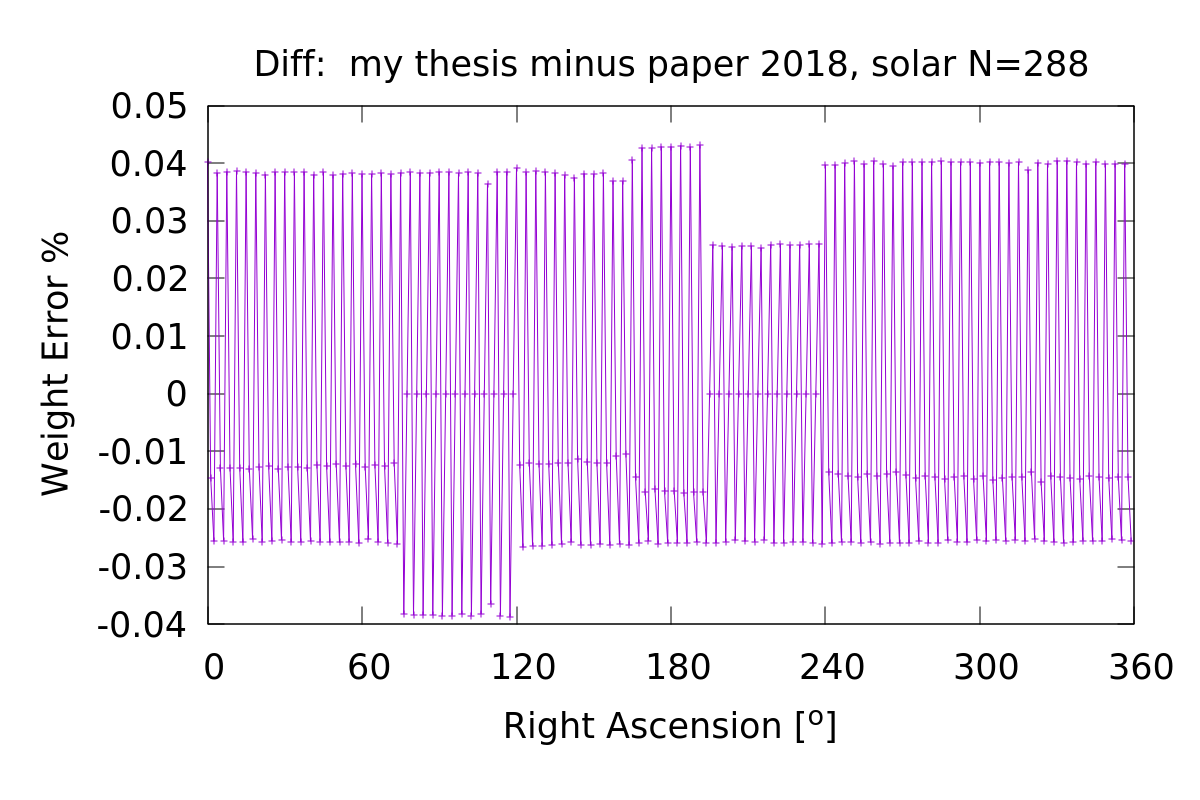
\includegraphics[width=0.45\textwidth]{solar_my_and_paper_in_288_error.png}
	\caption{Error porcentual de los pesos de la frecuencia solar con respecto al paper 2018.}
	\label{fig:error_288_solar}
\end{figure}

Para la frecuencia anti-sidérea no hay mucha diferencia a los obtenido para el caso de N=360. Los pesos se muestran en la Fig.\,\ref{fig:anti_288} y el error con respecto al valor del paper se muestra en la Fig.\,\ref{fig:error_288_anti}.

\begin{figure}[H]
	\centering
	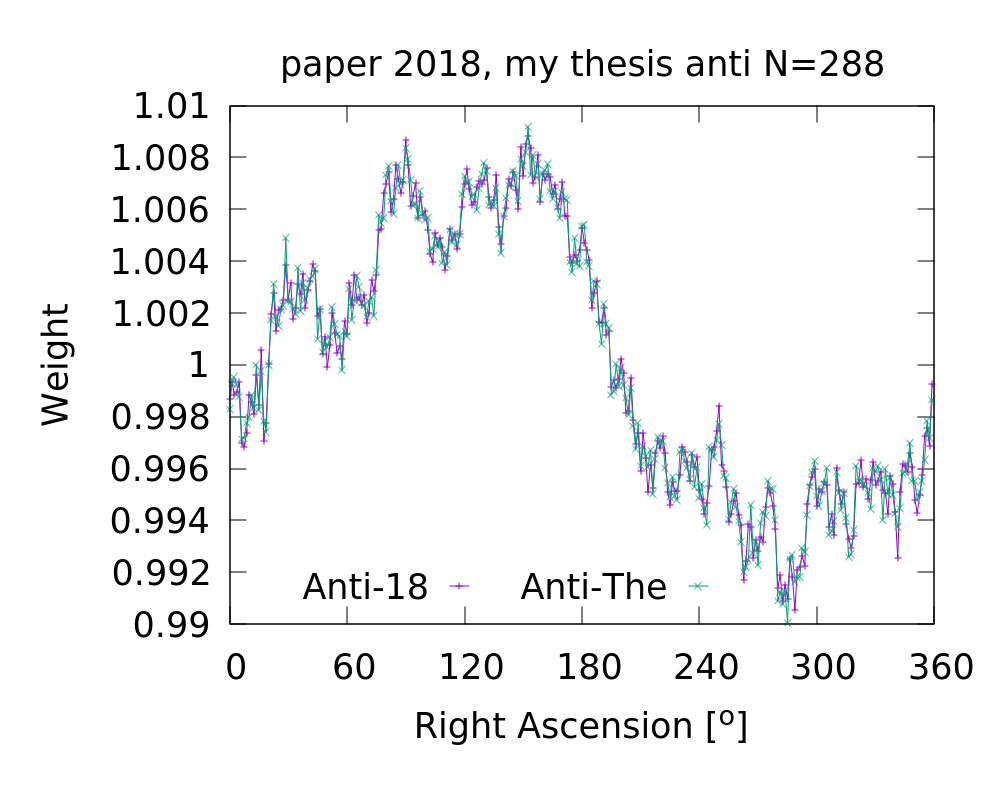
\includegraphics[width=0.45\textwidth]{anti_my_and_paper_2018_in_288.png}
	\caption{Pesos para la frecuencia anti-sidérea}
	\label{fig:anti_288}
\end{figure}


\begin{figure}[H]
	\centering
	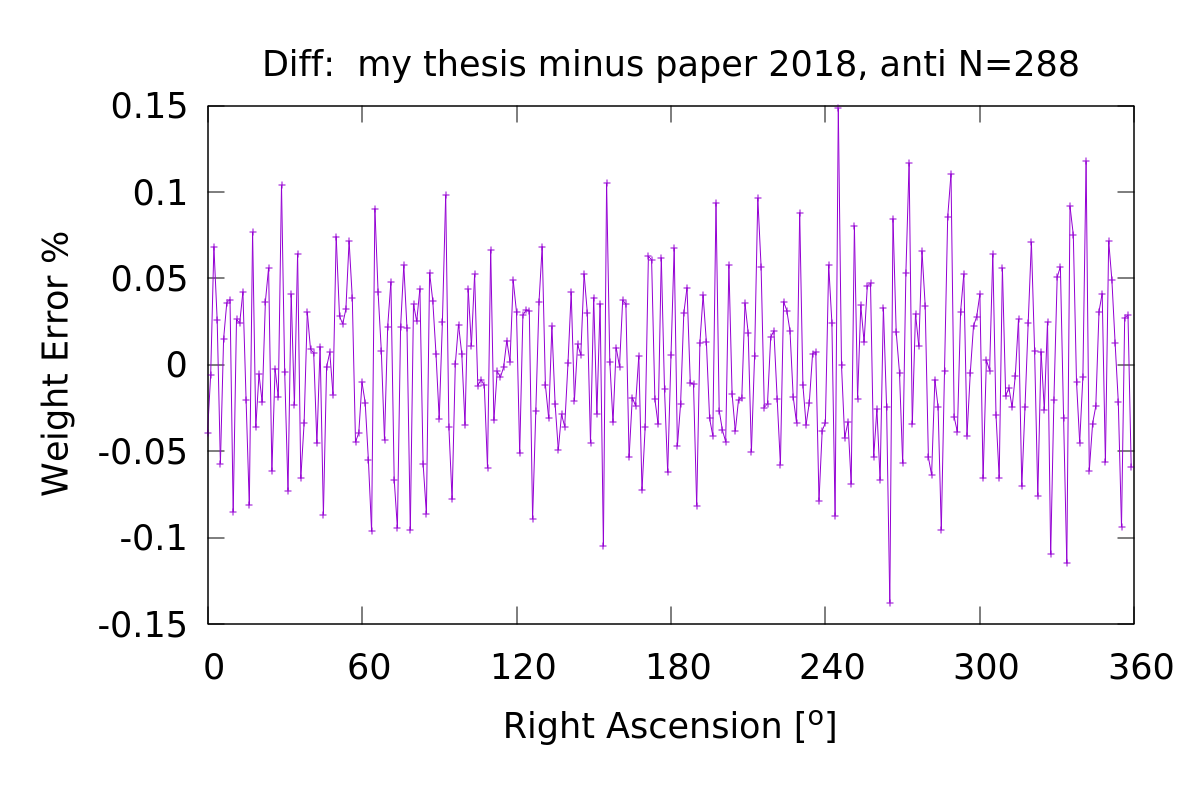
\includegraphics[width=0.45\textwidth]{anti_my_and_paper_in_288_error.png}
	\caption{Error porcentual de los pesos de la frecuencia anti-sidérea con respecto al paper 2018.}
	\label{fig:error_288_anti}
\end{figure}


\chapter{report 2 27 04 2020}
\graphicspath{{report_2_27_04_2020/}}
%\subsubsection{Nomenclatura}
%ai
%	\begin{table}[H]
%	\centering
%		\begin{tabular}{c|c|c|c}
%	Archivo AllTriggers  & \text{Eventos} & UTC inicial &  UTC final  \\ \hlineaiai
%	2020			 & 13 739 351	  &  1372680068	&  1577879983 \\ %2019
%	2019			 & 	8 463 063	  &	 1372680068 &  1496318388 \\ %Herald
%	2017			 &	8 592 302	  &  1372680068 &  1498521517 \\ %Oscar
%			\end{tabular}
%			\end{table}
%



\section{Anisotropías  considerando el peso de los hexágonos}

\subsection{Verificando que todo funcione como debe}


%Efectos espúreos: Por un lado estan esos piquitos chiquitos, que parecen ser algun problema numerico. Por otro hay todavia demasiados picos arriba de la linea de 99%.


%Se me ocurren dos checks que podrias hacer:

\subsubsection{Comparando con los datos de Oscar}
% 	1-  Uno, que tal vez ya hiciste, es correr tu programa en los datos que uso Oscar y ver de repetir los plots para las dos energias arriba de full efficiency (4-8 y >8)  para ver que el programa funciona igual

\begin{itemize}
	\item Agregar figuras sin peso 
	\begin{itemize}
		\item El de 4-8 para el 2017
		\item >8 para el 2017
	\end{itemize}
	\item buscar los valores de los dipolos conocidos y compararlos con lo que obtengo (usando los pesos)
\end{itemize}

\subsubsection{¿Análisis en frecuencia de los hexágonos?} \label{analisis_peso}
% 	2- Otra prueba que podrias hacer es hacer un  analisis en frecuencia  similar al que hiciste pero para la modulacion de hexagonos sola. Esto seria para ver que no hay cosas raras en el rate de hexagonos de estos datos. No tengo del todo claro como se haria. En vez de hacer la suma de senos y cosenos en los tiempos del zenit cuando llega un evento como ahora, habria que hacer esas sumas en un espaciado constante de tiempo (podrian ser los 5' en que estan bineados, y los pesos deberian ser proporcional a la cantidad de hexagonos. Pensalo un poco como se podria implementar y si queres lo charlamos despues.
\begin{itemize}
	\item ¿Barrido en frecuencia en ascensión recta?
	\item ¿Barriendo el archivo de eventos pero en vez de usar el evento para analizar, uso el valor del peso para el bin correspondiente? Suena bien.
\end{itemize}


%Hola, la fig 1 tiene en solar algunos saltos un poco raros. Podrias hacer esa misma figura (hexagonos en  solar, sidereo y antisidereo) para el periodo de tiempo desde 2004 a dic 2017 (asi comparamos con la comparacion que habian hecho Oscar y Ugo hace un tiempo.
%Y tambien hacela para el periodo completo hasta dic 2019, asi vemos lo que se usa para la ultima parte de tu documento.

\subsubsection{Comparando los pesos en sidérea, solar y antisiderea.}

Un ejemplo de como son los pesos para tres frecuencias en particular, para el rango 2013-2019, se muestra en la Fig.\,\ref{fig:pesos}


\begin{figure}[H]
	\centering
	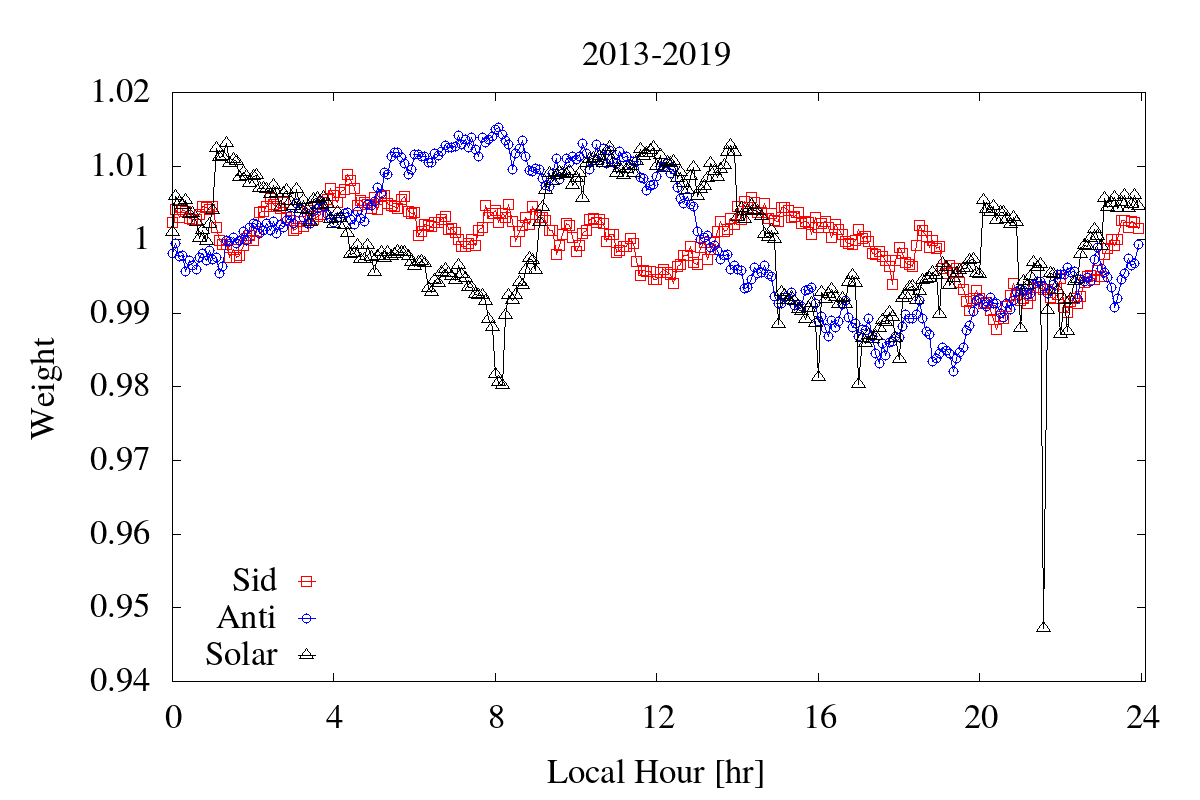
\includegraphics[width=0.5\textwidth]{weigth2013-2019.png}
	\caption{Pesos para las frecuencias sidérea, solar y anti-sidérea en el rango 2013-2019}
	\label{fig:pesos}
\end{figure}


Para el rango del 2004 hasta Jun 2017

\begin{figure}[H]
	\centering
	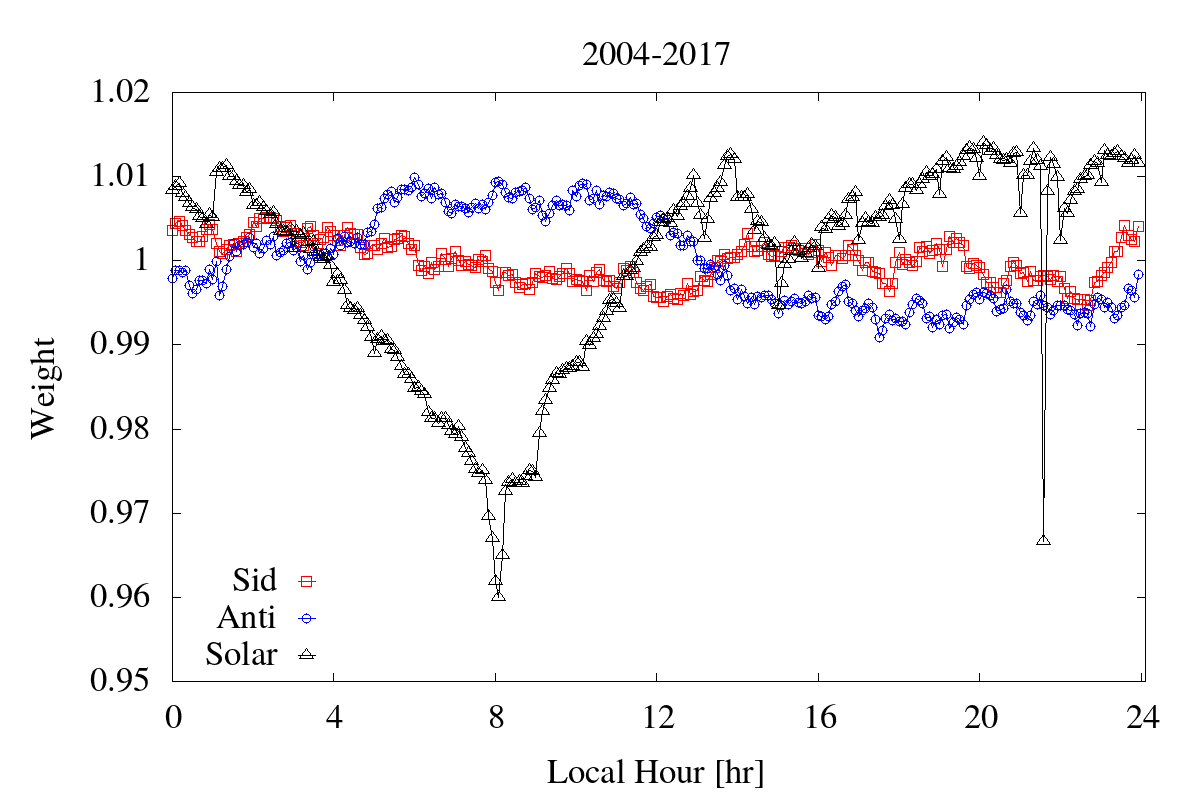
\includegraphics[width=0.5\textwidth]{weigth2004-2017.png}
	\caption{Pesos para las frecuencias sidérea, solar y anti-sidérea en el rango 2004-2017}
	\label{fig:pesos_2017}
\end{figure}



Para el rango entre el $2005$ y $2019$
\begin{figure}[H]
	\centering
	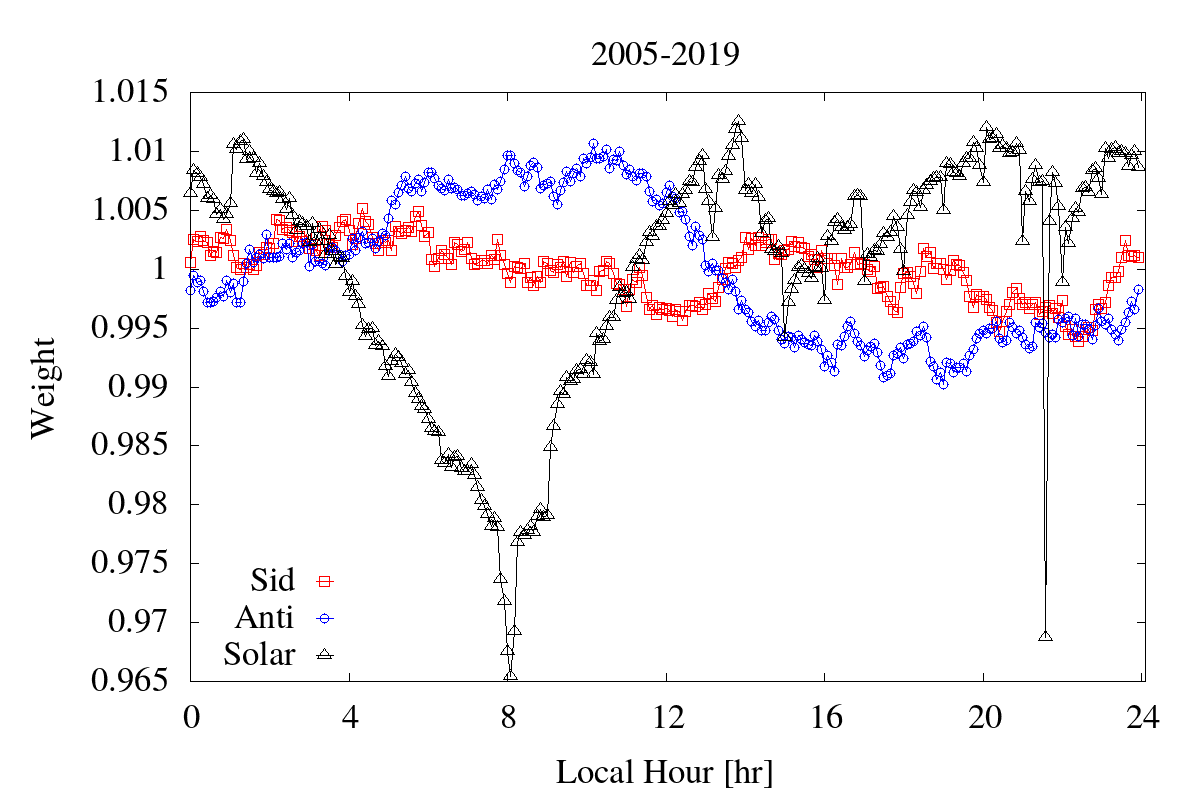
\includegraphics[width=0.5\textwidth]{weigth2005-2019.png}
	\caption{Pesos para las frecuencias sidérea, solar y anti-sidérea en el rango 2005-2019}
	\label{fig:pesos_2019}
\end{figure}




La idea que tengo sobre el pico en ambos gráficos es algo en la cantidad de hexagonos, algún periodo donde se apagó la mitad del observatorio o algo así. Quiero hacer la evolución de la cantidad de hexagonos para ese bin en particular en la frecuencia. Estaba pensando en como codearlo para que me sirva también para hacer \ref{analisis_peso}.


%Otra cosa, en general: seria bueno hacer los plots entre 363.25 y 367.25 (ya que las tres que nos interesan son 364.25, 365.25 y 366.25). PARA DESPUÉS
%Otra curiosidad, en frecuencia siderea, cual es la fase en RA y la probabilidad del bin entre 1y 2?


\subsection{Variación de los pesos en función de la ascensión recta}
En las figuras de esta sección se muestran el análisis en ascensión recta para los eventos de observatorio considerando las variaciones de la exposición. 
Los mismos se hicieron en el mismo intervalo de tiempo para poder compararlos entre sí. Elegí el rango presentado en la Tabla \ref{rango_corto}  porque en el mismo se encuentran todos los eventos filtrados por energía, por bad period, por reconstrucción correcta, etc. El rango empieza en el 2013 porque la última versión del archivo de todos los disparos empezó a registrarse desde el  1 de Julio del 2013 a las 12:01:08 GMT (1372680068) hasta el  1 de enero del 2020 a las 11:59:43 (1577879983). Mientras que el archivo del disparo estándar va desde el 01 de enero del 2004.

	\begin{table}[H]
	\centering
		\begin{tabular}{c|c|c|c}
	 		& UTC 			& Fecha		 	&  Hora GMT  \\ \hline
	Inicio	& 1372699409	&2013-07-01 	&17:23:29		\\
	Final 	& 1577825634	&2019-12-31 	&20:53:54		\\
		\end{tabular}
	\caption{Rango de tiempo considerando todos los disparos} 	\label{rango_corto}
	\end{table}


\subsubsection{Energía entre 1\,EeV y 2\,EeV}

Para este caso utilizamos el archivo con todos los disparos en el rango de energía $1\,$ EeV - $2\,$EeV donde se tiene $1\,321\,702$ eventos.

\begin{figure}[H]
	\centering
	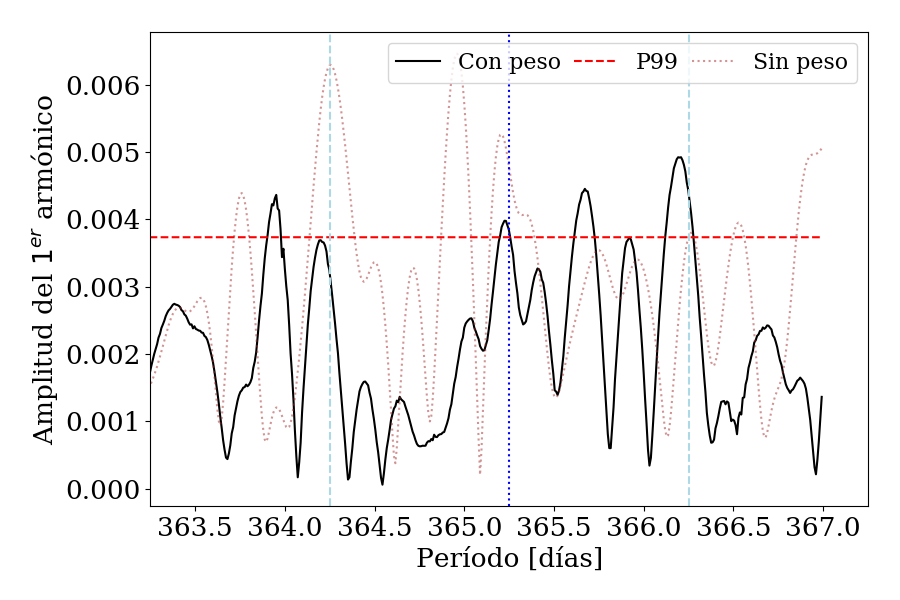
\includegraphics[width=0.5\textwidth]{2019_AllTriggers_1_2_EeV_con_vs_sin_peso.png}
	\caption{Todos los disparos: entre 1 EeV y 2 EeV, entre 2013-2019}
	\label{fig:12w}
\end{figure}
%fig

\emph{Otra curiosidad, en frecuencia siderea (366.25), cual es la fase en RA y la probabilidad del bin entre 1y 2?}

La siguiente tabla se había calculado usando la formula 

\begin{equation}
	\tilde \alpha = 2\pi \frac{t_i}{T_x} +\alpha_i - \alpha^0
\end{equation}
donde $\alpha_i$ y $\alpha^o$ con las RA del evento y del cenit del observatorio.

	\begin{table}[H]
	\centering
		\begin{tabular}{c|c}
	 		&  2013-2019 (Con peso)	 \\ \hline
	Fase		& 	306.611				 \\
	$r$ 		&  0.00440897			\\
	$r_{99}$ 	&  0.00373348			\\
	$P(\tilde r)$ 	    & 	0.162485	\%	 \\
		\end{tabular}
	\caption{Rango de tiempo considerando todos los disparos} 	\label{rango_corto}
	\end{table}


\subsubsection{Energía entre 2\,EeV y 4\,EeV}

Para este caso utilizamos los eventos del archivo con todos los disparos con energía entre $2\,$ EeV - $4\,$EeV, donde se encontraron $288\,444$ eventos.
\begin{figure}[H]
	\centering
	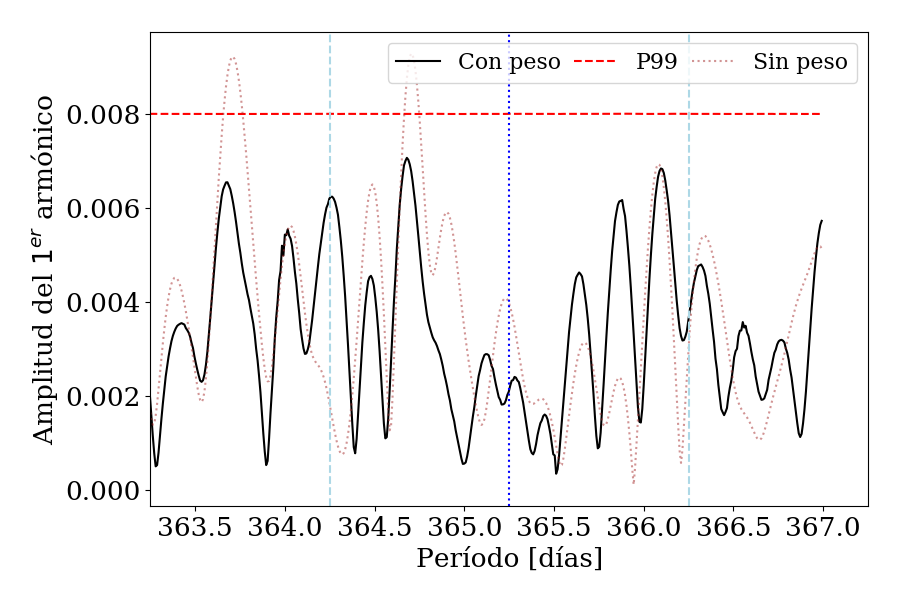
\includegraphics[width=0.5\textwidth]{2019_AllTriggers_2_4_EeV_con_vs_sin_peso.png}
	\caption{Todos los disparos: entre 2 EeV y 4 EeV, entre 2013-2019}
	\label{fig:24w}
\end{figure}

En la Fig.\,\ref{fig:24w} no se ve ningún pico por encima de  percentil 99.


\subsubsection{Energía entre 4\,EeV y 8\,EeV}

A partir de $3\,$EeV el disparo estándar tiene una eficiencia del $100\%$. Entonces para este  intervalo de energías,  utilizamos el archivo con el disparo estandar.

\begin{figure}[H]
	\centering
	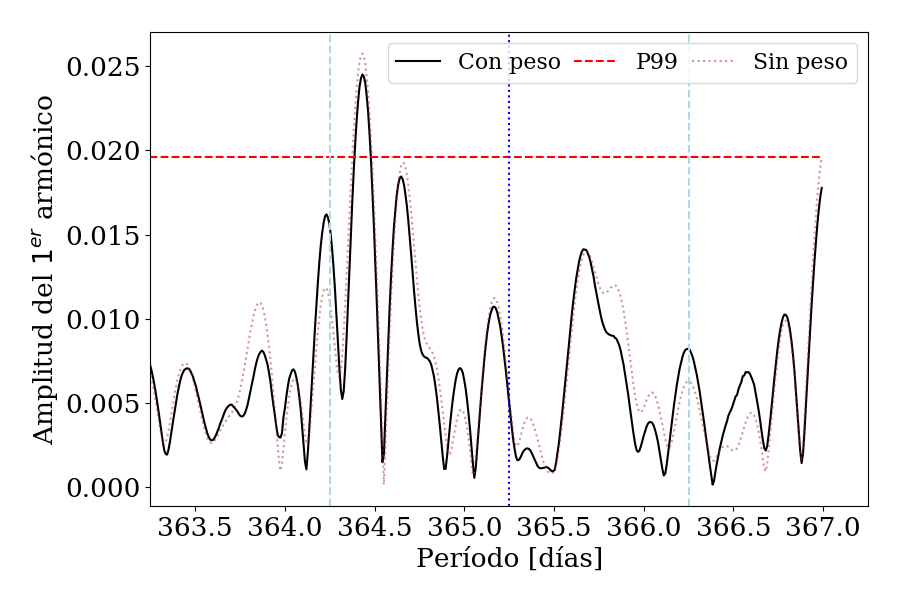
\includegraphics[width=0.5\textwidth]{2019_Main_Array_4_8_EeV_con_vs_sin_peso.png}
	\caption{Disparos estándar: entre 4 EeV y 8 EeV, entre 2013-2019}
	\label{fig:48w}
\end{figure}
%fig

\subsubsection{Energía sobre 8\,EeV}

Para este caso utilizamos el archivo con el disparo estandar

\begin{figure}[H]
	\centering
	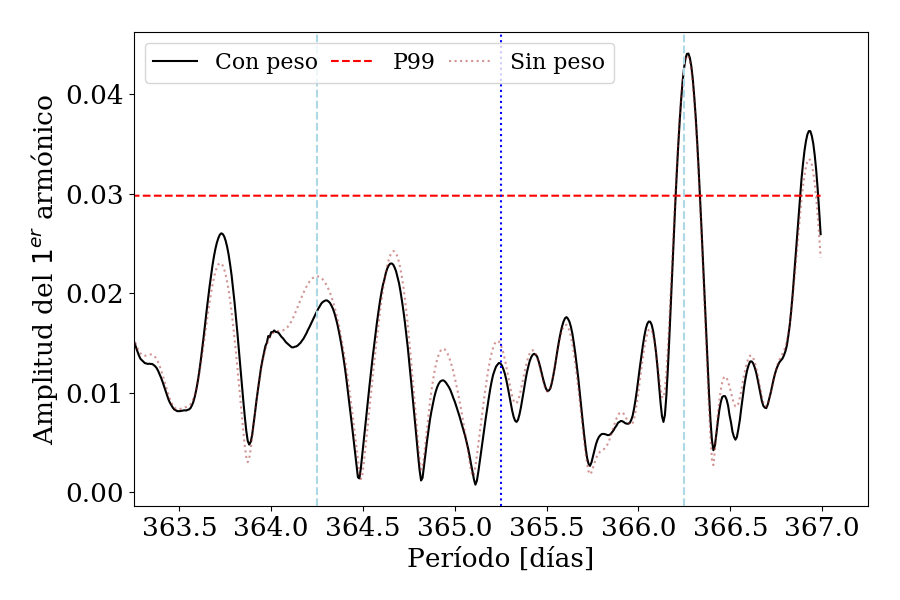
\includegraphics[width=0.5\textwidth]{2019_Main_Array_8_EeV_con_vs_sin_peso.png}
	\caption{Disparos estándar: encima de 8 EeV, entre 2013-2019}
	\label{fig:8w}
\end{figure}
%fig




\subsection{Ampliando el rango de tiempo para el archivo del disparo estándar}

Amplié el rango de tiempo para poder compararlo con los gráficos anteriores, ya que se espera que mientras mayor sea el rango de tiempo los efectos espúreos disminuyen.

	\begin{table}[H]
	\centering
		\begin{tabular}{c|c|c|c}
	 		& UTC 			& Fecha		 	&  Hora GMT  \\ \hline
	Inicio	& 1104537600	&2005-01-01 	&00:00:00		\\
	Final 	& 1577825634	&2019-12-31 	&20:53:54		\\
		\end{tabular}
	\end{table}


\subsubsection{Energía entre 4\,EeV y 8\,EeV}

\begin{figure}[H]
	\centering
	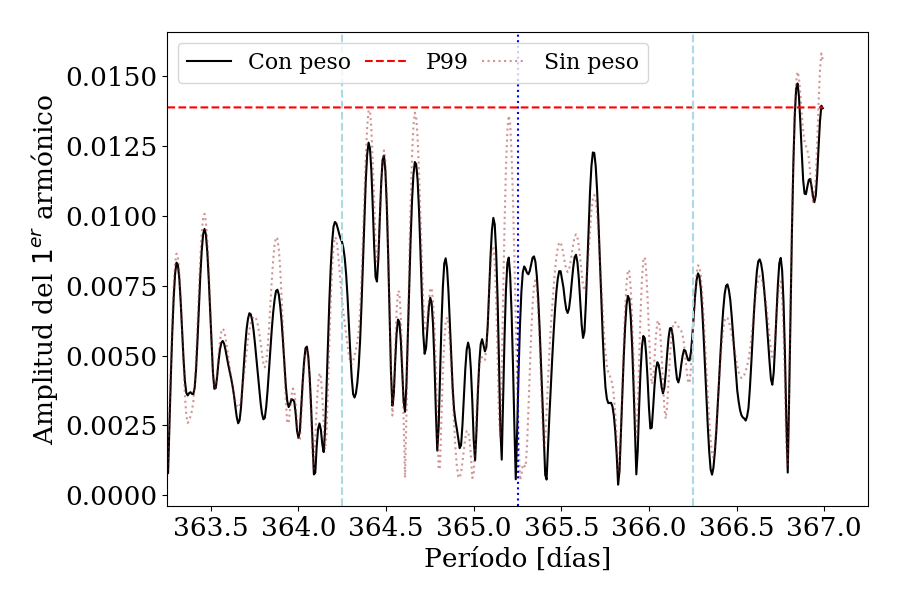
\includegraphics[width=0.5\textwidth]{2019_Main_Array_4_8_EeV_con_vs_sin_peso_extended.png}
	\caption{Disparos estándar: entre 4 EeV y 8 EeV extendiendo el rango hasta el 2005}
	\label{fig:48w_extended}
\end{figure}
%fig

\subsubsection{Energía sobre 8\,EeV}


\begin{figure}[H]
	\centering
	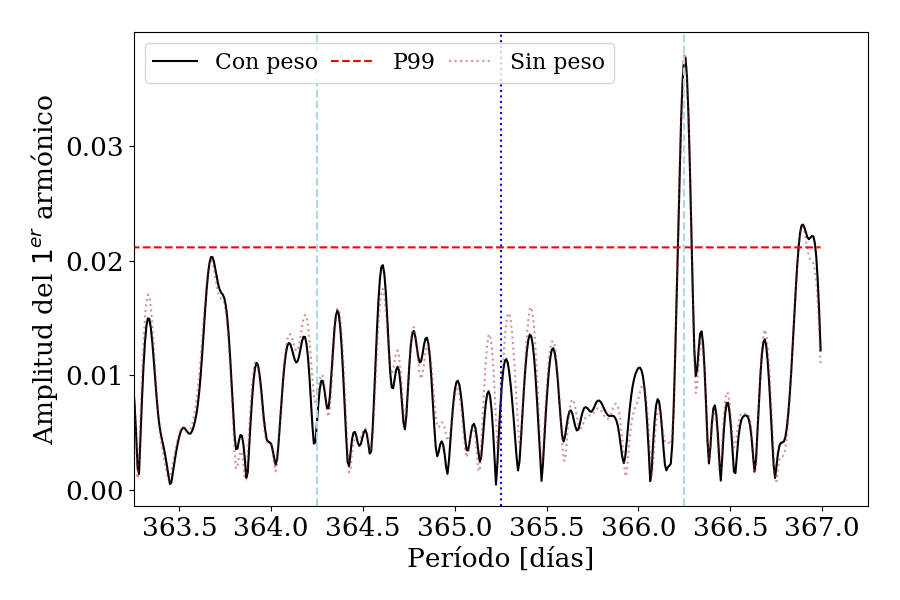
\includegraphics[width=0.5\textwidth]{2019_Main_Array_8_EeV_con_vs_sin_peso_extended.png}
	\caption{Disparos estándar: encima de 8 EeV extendiendo el rango hasta el 2005}
	\label{fig:8w_extended}
\end{figure}
%fig

\chapter{report 3 07 05 2020}
\graphicspath{{report_3_07_05_2020/}}


\subsection{Rango de tiempo}
\begin{table}[H]
\centering
\begin{tabular}{c|c|c}
Inicio & 1388628499 & 2 January 2014 \\ \hline
Final  & 1550534100 & 18 February 2019 \\
\end{tabular}
\end{table}

\subsection{Tasa de eventos}

\begin{figure}[H]
	\centering
	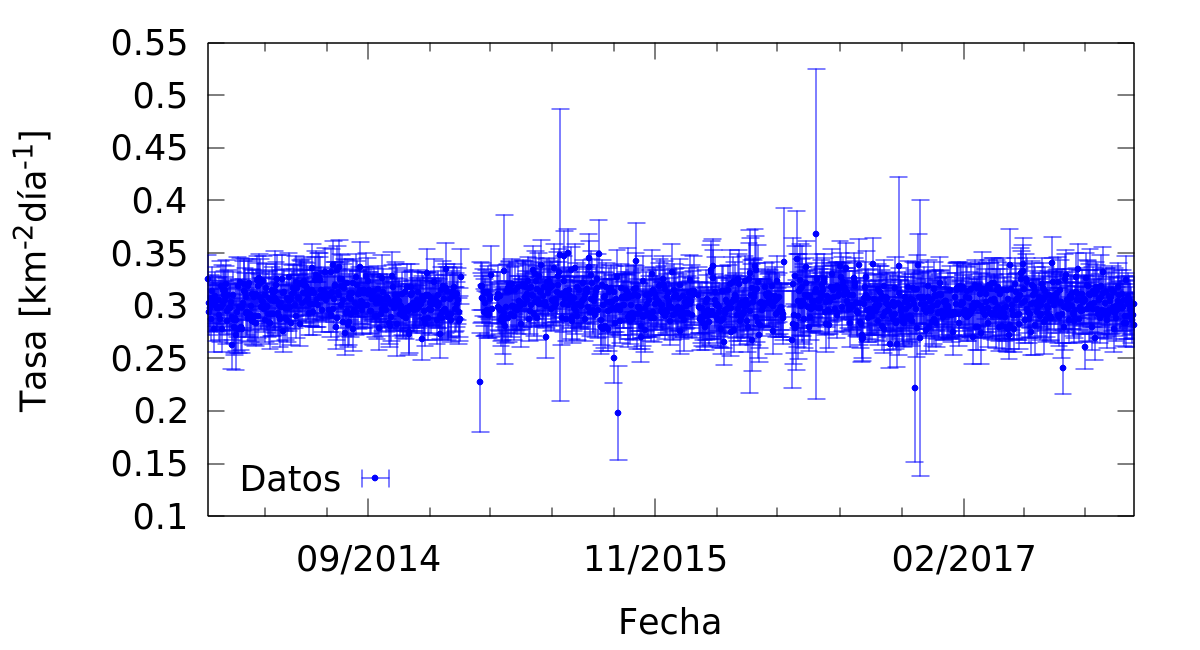
\includegraphics[width=0.5\textwidth]{rate_1_EeV.png}
	\caption{Tasa de eventos para eventos por encima de 1 EeV.}
\end{figure}

Antes del 2 de Enero del 2014, se tenía una tasa por debajo de la media de los siguientes años.

La cantidad de hexágonos 6T5 durante el periodo mencionado arriba evolucionó como se muestra  en la figura que sigue


\begin{figure}[H]
	\centering
	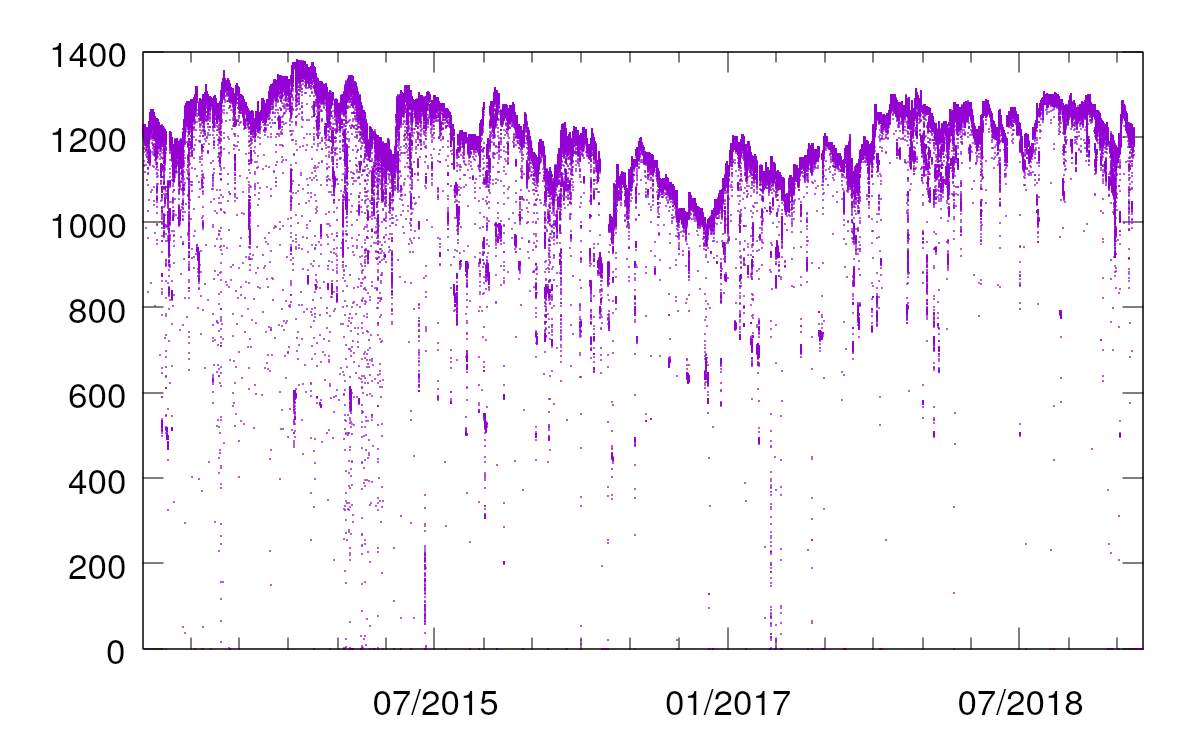
\includegraphics[width=0.5\textwidth]{hex_rango_corto.png}
	\caption{Hexágonos}
\end{figure}


\subsection{Párametros del clima}

\begin{figure}[H]
	\centering
	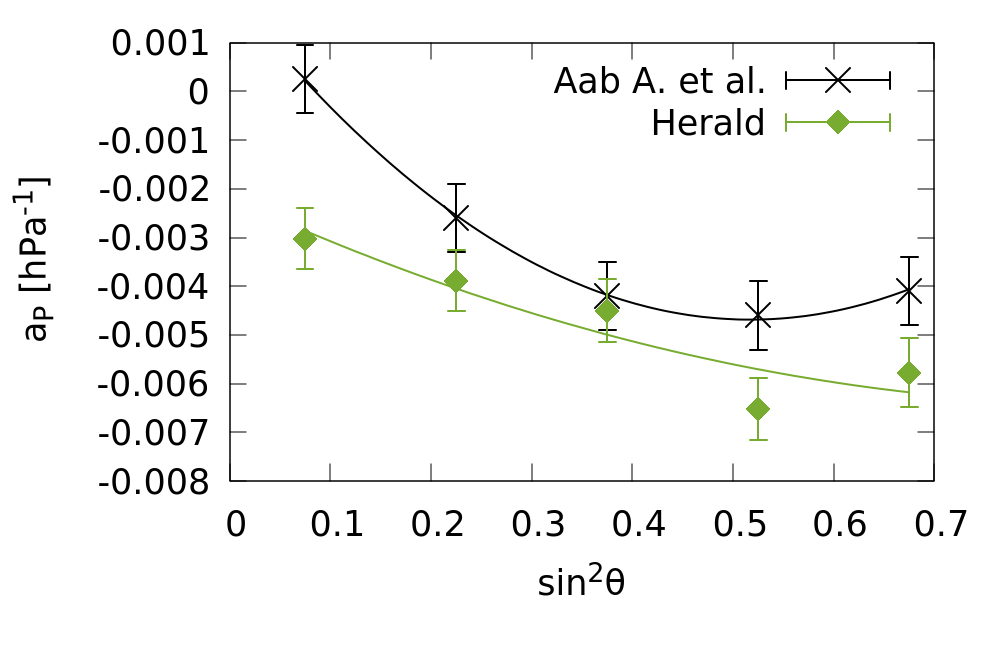
\includegraphics[width=0.5\textwidth]{ap.png}
\end{figure}


\begin{figure}[H]
	\centering
	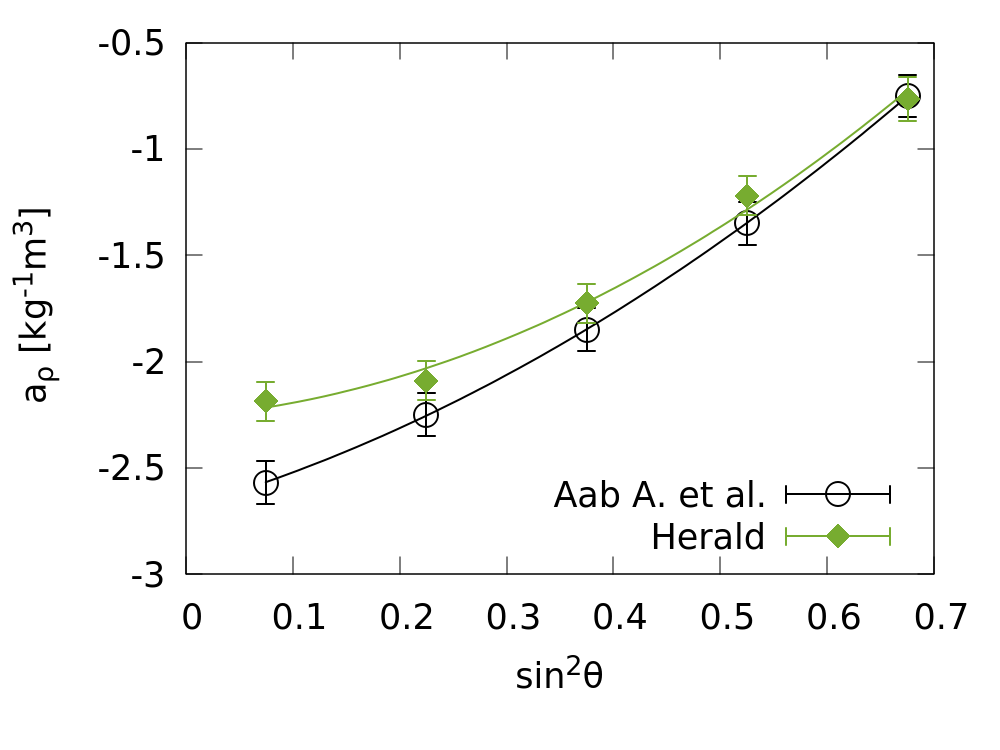
\includegraphics[width=0.5\textwidth]{arho.png}
\end{figure}


\begin{figure}[H]
	\centering
	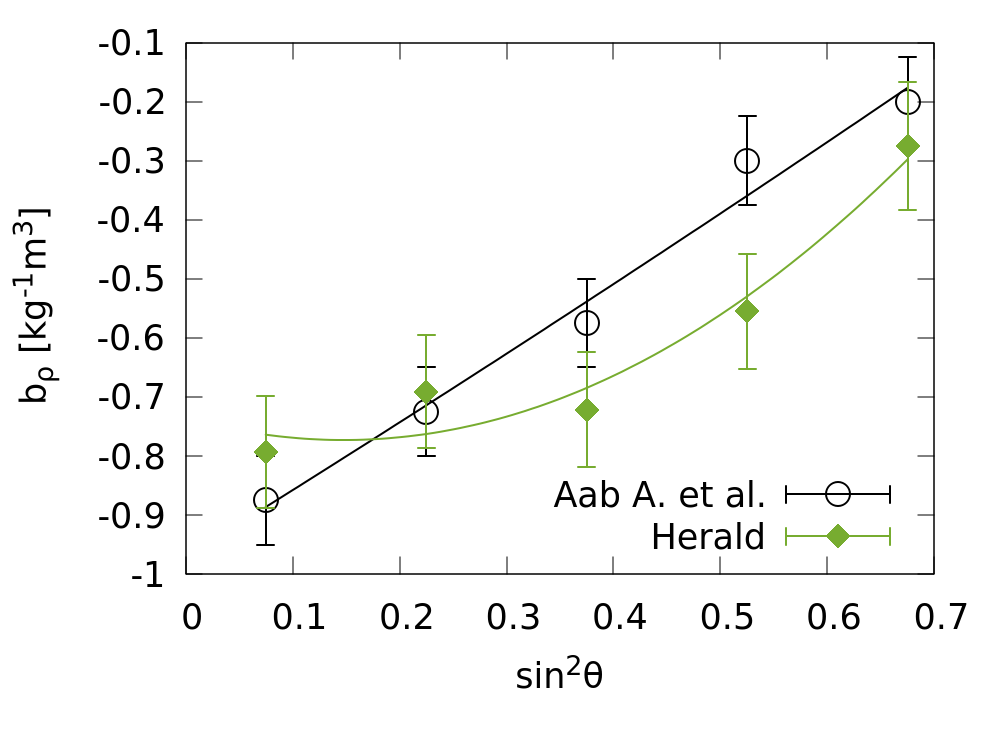
\includegraphics[width=0.5\textwidth]{brho.png}
\end{figure}




Considerando una cuádrica para el ajuste de la curva, se obtiene los parámetros de la siguiente table
\begin{table}[H]
\centering
\begin{tabular}{c|c|c|c}
		 	& $a_P$ 	&  $a_\rho$  & $ b_\rho$ \\ \hline
$c_0$ 		& -0.002(1) & 	-2.2(1)	 &	-0.74(9)\\ \hline
$c_1$ 		& -0.009(6)	& 	 0.4(6)	 &	-0.0(6)\\ \hline
$c_2$ 		&  0.00(9) 	& 	 2.7(8)  &	 1.7(7)\\ \hline
\end{tabular}
\end{table}


\subsection{Anisotropía en el rango 1-2 EeV}

\begin{figure}[htbp]
	\centering
	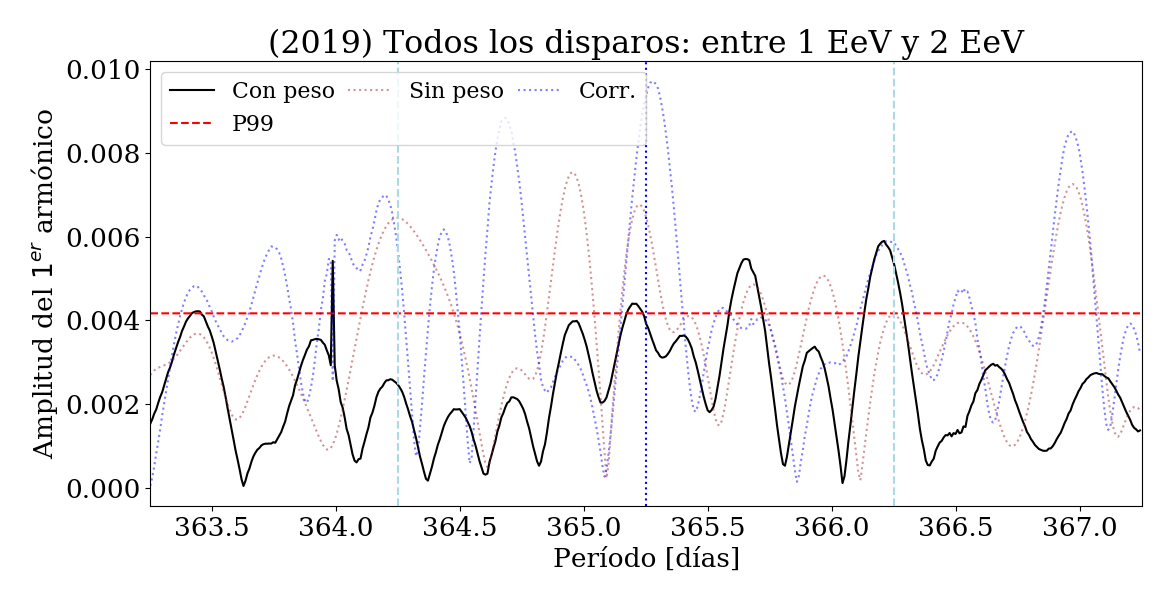
\includegraphics[width=0.5\textwidth]{ani_corr.png}
\end{figure}


\chapter{report 4 12 05 2020}
\graphicspath{{report_4_12_05_2020/}}

La selección de los eventos genera dos conjuntos de datos: uno para el análisis de anisotropía en el bin 1 EeV - 2 EeV, y el segundo de los eventos con energía mayor a 1 Eev para obtener los parámetros del clima. En esta selección se tiene en cuentan los eventos de $\theta < 60^o$ \footnote{el archivo que bajo de \url{http://ipnwww.in2p3.fr/~augers/AugerProtected/herald.php} }, como también  los mismos que no se encuentren en un periodo de mala adquisición datos, este parámetro se denomina $ib$ de los \textbf{eventos del herald}. Este periodo consiste en momento donde el obsevatorio no recibe datos de las estaciones de clima o de los hexágonos. 

El parámetro de $ib$ de los \textbf{datos del clima} es irrelevante durante el proceso de filtrar eventos. Entra en juego cuando hago el análisis del clima, donde desecho los eventos que fueron recabados durante \emph{bad weather} \textbf{y} no fueron filtrados ya antes. 


\section{Pesos de los hexágonos}

Para constatar que no exista ninguna anomalía en los pesos de los hexágonos, se realiza el cálculo de los mismos para tres frecuencias de referencia para el análisis de anisotropías.  Los pesos se muestran en la Fig.\,\ref{fig:wei_14_20}. El rango de tiempo en el que se calculan estas curvas es entre 1 de Enero del 2014 y el 1 de Enero del 2020.

\begin{figure}[H]
	\centering
	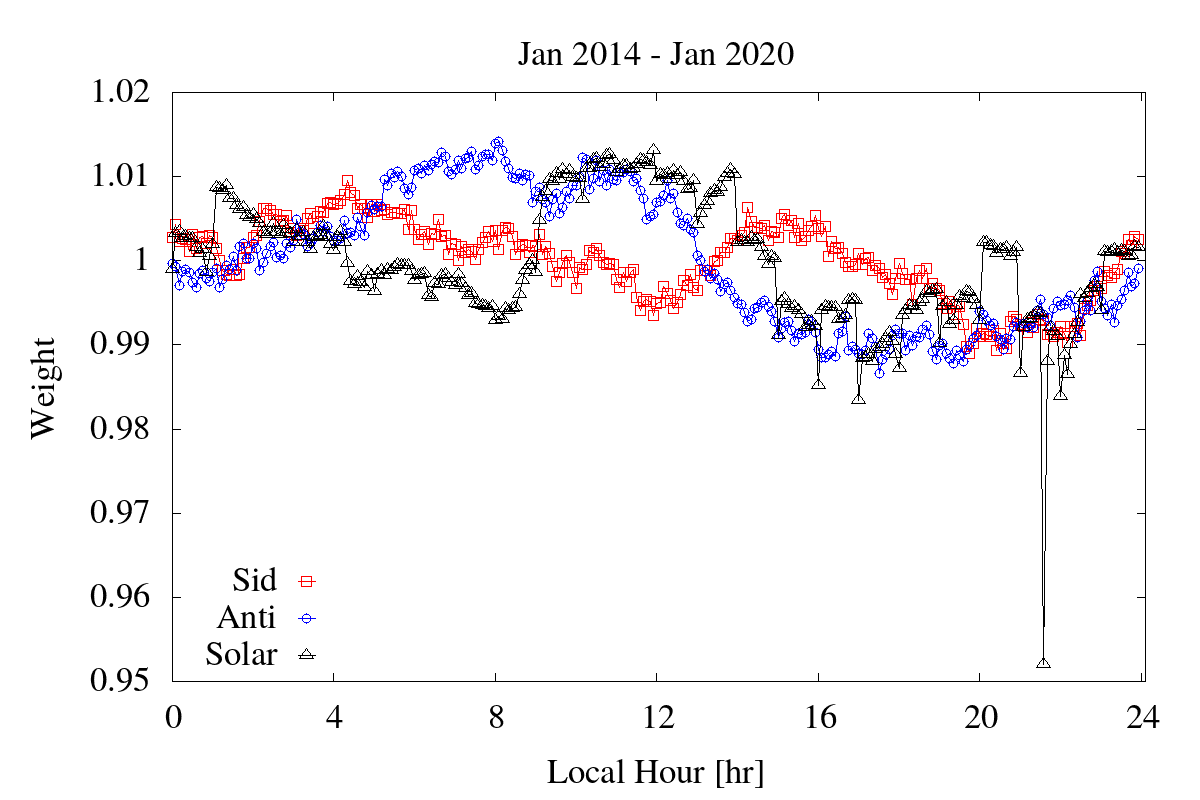
\includegraphics[width=0.5\textwidth]{weigth2014-2020_jan.png} 	
	\caption{Pesos de los hexágonos}
	\label{fig:wei_14_20}
\end{figure}

\section{Anisotropía}
El archivo de de todos los disparon empieza el Mon, 1 July 2013 12:05:08 GMT \footnote{$1372680308$}. Para trabajar en una cantidad entera de años, se trabaja a partir del  Thur, 1 January 2014 12:00:00 GMT \footnote{$1388577600$} y hasta el Thursday, 1 January 2020 12:00:00 GMT \footnote{$1577880000$}.  En este rango se tiene la tasa de eventos por día que se muestra en la Fig.\,\ref{tasa_total_diaria}.

% En el rango $1372680308$ \footnote{Mon, 1 July 2013 12:05:08 GMT} y $1388577600$ \footnote{Thur, 1 January 2014 12:00:00 GMT}, la tasa de eventos del archivo $\text{All Triggers}$, tenía una tasa de eventos por debajo de lo normal. Por esto, se utiliza los eventos a partir del  1388577600. La tasa de eventos que se utiliza se puede ver a continuación:

\begin{figure}[H]
	\centering
	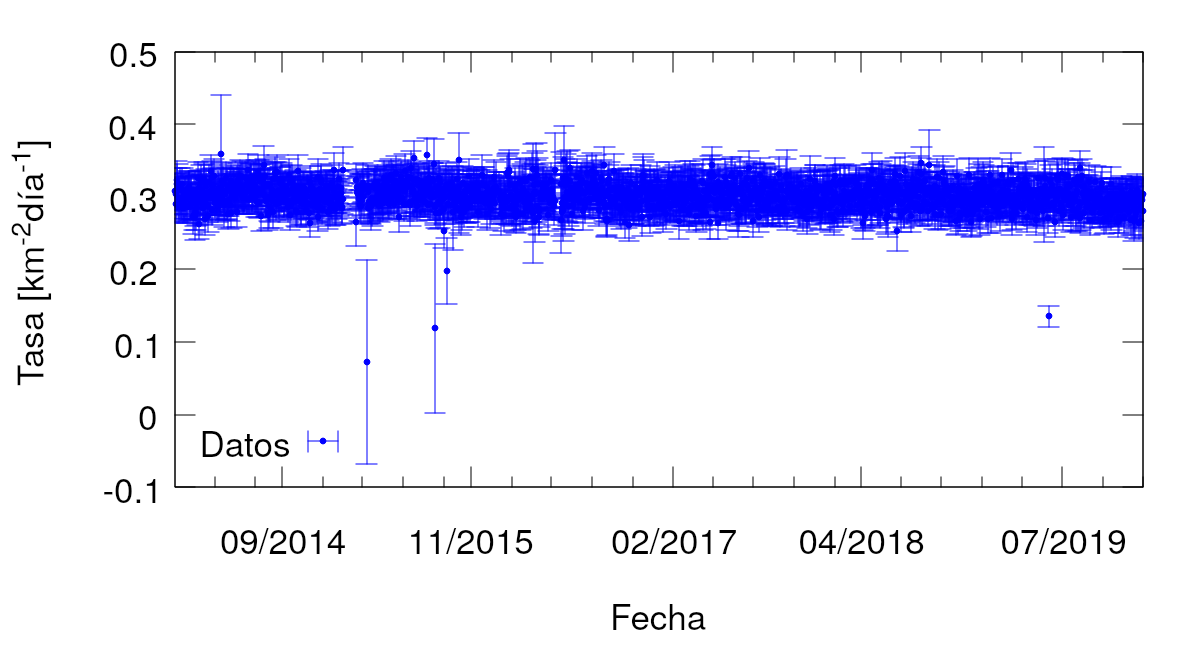
\includegraphics[width=0.5\textwidth]{rate_total.png}
	\caption{Tasa  de eventos en el rango de tiempo a trabajar}
	\label{tasa_total_diaria}
\end{figure}

\subsection{Lista detallada de los filtros aplicados de datos del herald}

\subsubsection{Datos para el análisis de anisotropía}
Esta sección muestra los filtros para los datos del análisis de anisotropía en el rango 1 EeV - 2 EeV.

\begin{enumerate}
	\item Energía entre  [1 EeV , 2 EeV)
	\item Rango de tiempo:
	\begin{itemize}
		\item[-] Inicial:1388577600 \\ (Thursday, 1 January 2014 12:00:00 GMT)
		\item[-] Final: 1577880000  \\ (Thursday, 1 January 2020 12:00:00 GMT)
	\end{itemize}
	\item Sectancia:  $\theta < 60^o$
	\item 6T5
	\item $ib=1$ Bad period flag. Un valor de 1 indica un buen periodo
\end{enumerate}

Con estos filtros se tienen $1\,092\,753$ eventos

\subsubsection{Datos para el cálculo de las correcciones del clima}

Estos son los filtros para los datos a utilizar para el cálculo de los parámetros del clima:

\begin{enumerate}
	\item Eventos con valor de señal de $S_{38}$\footnote{Valor de S38 sin la correccón del clima del paper del 2017} por encima de  $5.36\,\text{VEM}$. Este valor corresponde a $\sim 1\,$ EeV  en VEM.
	\item Rango de tiempo:
	\begin{itemize}
		\item[-] Inicial:1388577600 \\ (Thursday, 1 January 2014 12:00:00 GMT)
		\item[-] Final: 1577880000  \\ (Thursday, 1 January 2020 12:00:00 GMT)
	\end{itemize}
	\item Sectancia:  $\theta < 60^o$
	\item $iw<4$ (weather quality flag)
	\item 6T5
	\item $ib=1$ Bad period flag del herald.  Un valor de 1 indica un buen periodo
	\item $ib=1$ Bad period flag de los datos del clima. Un valor de 1 indica un buen periodo
\end{enumerate}


Con estos filtros se tienen $1\,208\,615$ eventos, con una tasa de eventos que se muestra en la Fig.\,\ref{tasa_total_diaria_ajuste_weather}. En la figura se observa que utilizando el corte en la señal de S38 sin corregir por la modulación del clima del herald \footnote{Las correcciones se calcularon para el archivo del disparo estándar} se observa una modulación anual.

\begin{figure}[H]
	\centering
	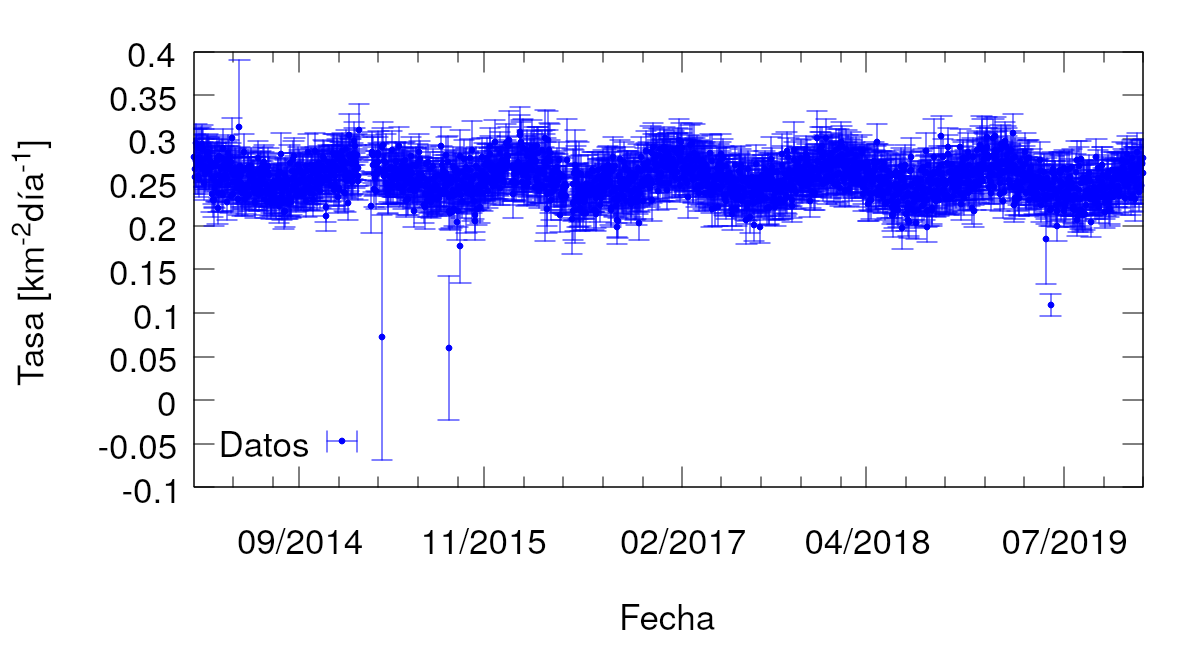
\includegraphics[width=0.5\textwidth]{rate_total_ajuste_weather.png}
	\caption{Tasa  de eventos en el rango de tiempo a trabajar para el ajuste de los parámetros del clima.}
	\label{tasa_total_diaria_ajuste_weather}
\end{figure}


\subsection{Análisis en frecuencia}

\begin{figure}[H]
	\centering
	\includegraphics[width=0.5\textwidth]{2019_AllTriggers_1_2_EeV_con_vs_sin_peso.png}
	\caption{Análisis en frecuencia en ascensión recta en rango 1 EeV - 2 EeV}
	\label{fig:consin}
\end{figure}


\section{Corrección del clima}

\begin{figure}[H]
	\centering
	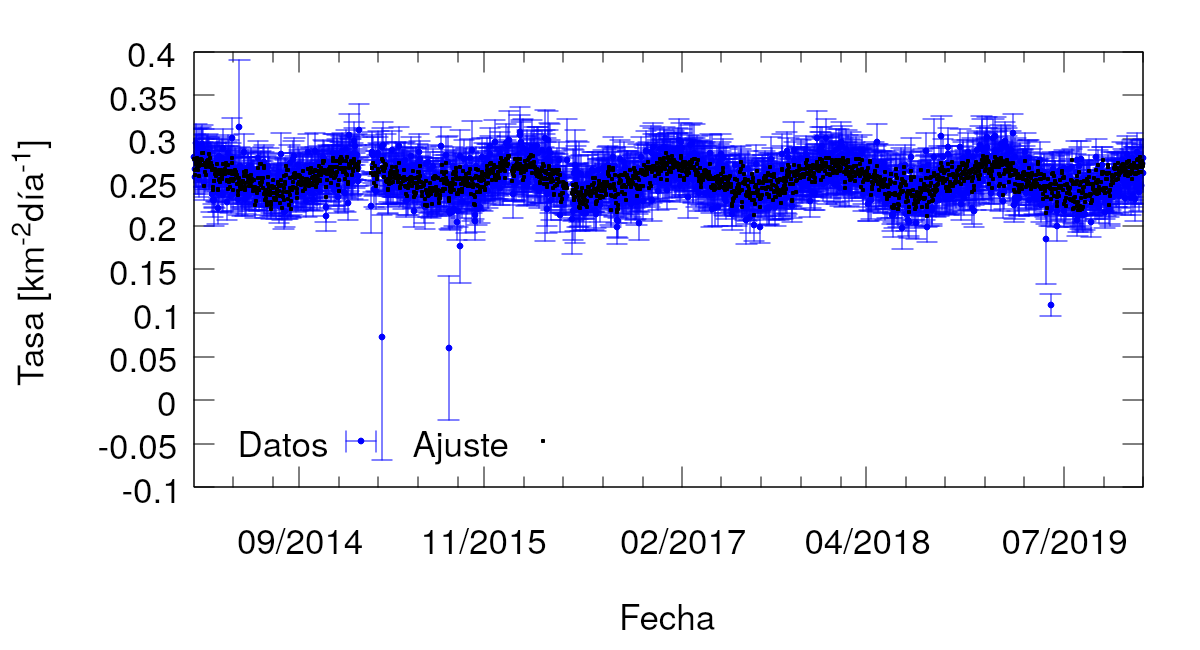
\includegraphics[width=0.5\textwidth]{rate_Ajuste.png}
\end{figure}



\begin{figure}[H]
	\centering
	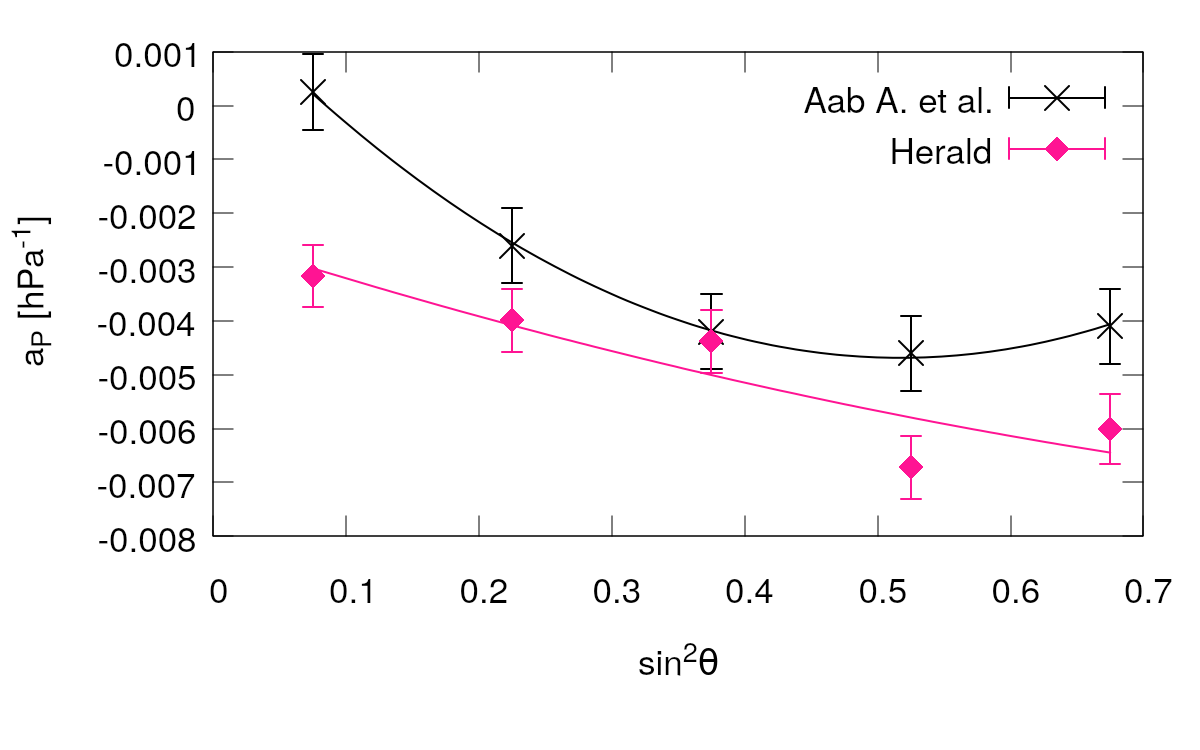
\includegraphics[width=0.5\textwidth]{ap_6t5.png}
	\caption{Parámetro de clima $a_P$ calculado para la corrección del archivo de todos los disparos}
\end{figure}

\begin{figure}[H]
	\centering
	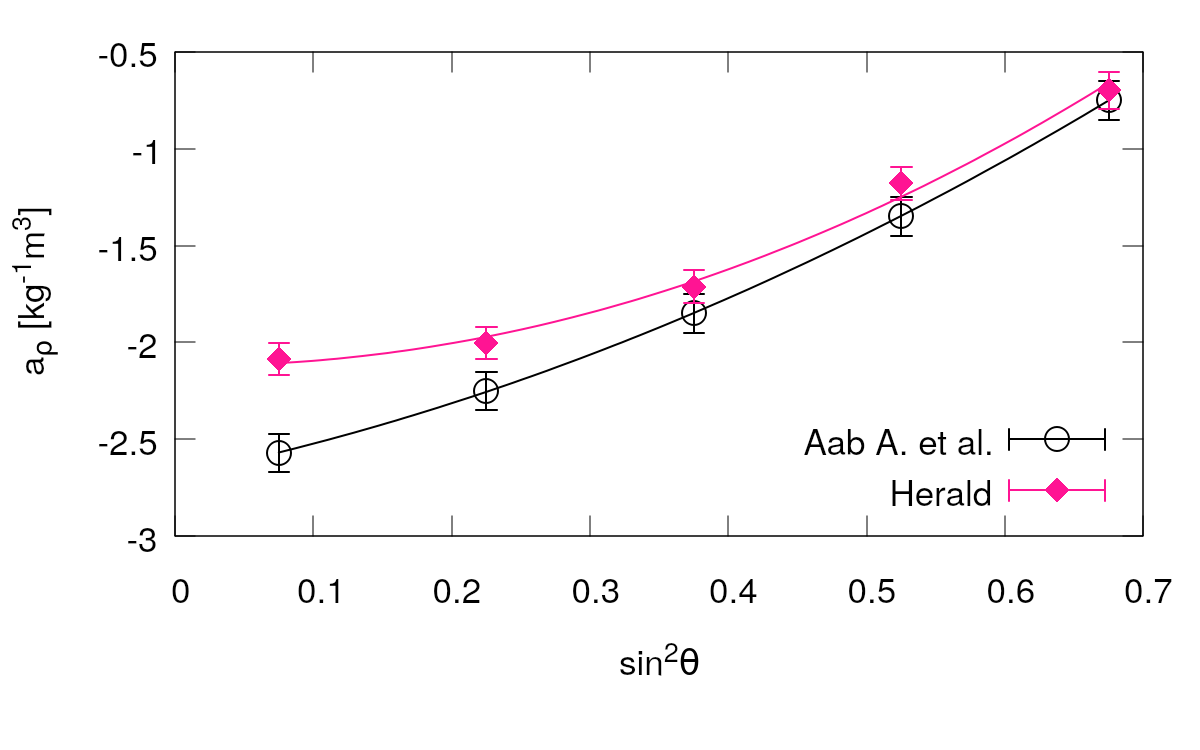
\includegraphics[width=0.5\textwidth]{arho_6t5.png}
	\caption{Parámetro de clima $a_\rho$ calculado para la corrección del archivo de todos los disparos}
\end{figure}

\begin{figure}[H]
	\centering
	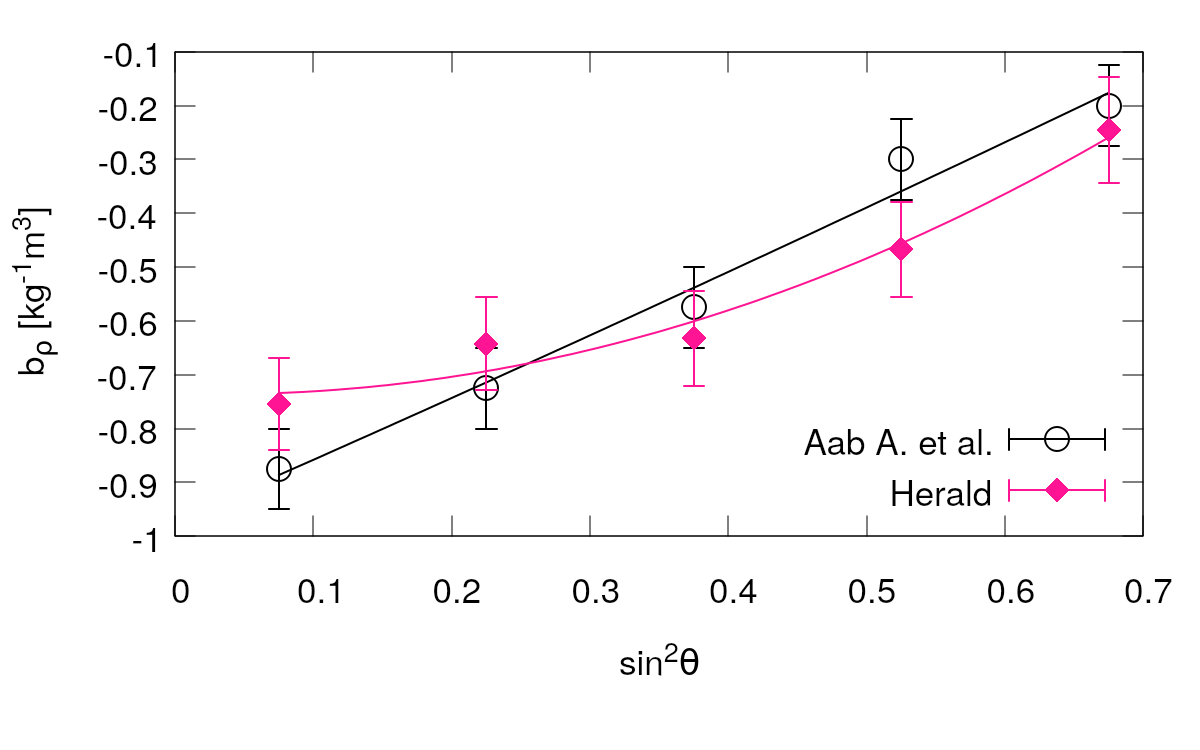
\includegraphics[width=0.5\textwidth]{brho_6t5.png}
	\caption{Parámetro de clima $b_\rho$ calculado para la corrección del archivo de todos los disparos}
\end{figure}



\chapter{report 5 22 05 2020}
\graphicspath{{report_5_22_05_2020/}}
\section{Anisotropías  }
\begin{table}[H]
\centering
\begin{tabular}{l|c|c}
				& Con Peso 	& Sin peso 		\\ \hline
Frecuencia:		& 366.25 	& 366.25 		\\
Fase:			& 329.865 	& 292.312		\\
$P_{99}$:		& 0.76398\%	& 26.6838 \% 	\\
$r_{99}$:		& 0.004676 	& 0.00243515	\\
\end{tabular}
\caption{Fase, $r_{99}$ y $P_{99}$ del análisis de anisotropía entre en 1 de Enero del 2014 y el 1 de Enero del 2020}
\end{table}


\begin{figure}[H]
	\centering
	\includegraphics[width=0.8\linewidth]{../report_4_12_05_2020/2019_AllTriggers_1_2_EeV_con_vs_sin_peso.png}
	\caption{Anisotropía para el intervalo 2014-2020}
	\label{fig:anis}
\end{figure}

En la Fig.\ref{fig:zoom} se muestra el pico que se presenta en  el intervalo de energía entre 1 EeV - 2 EeV, cercano a la frecuencia sidérea. El pico tiene un máximo para un período de $366.21$. En la Tabla.\,\ref{tabla:pico} se muestran los valores de la fase, $r_{99}$ y $P_{99}$ para el periodo anterior.

\begin{figure}[H]
	\centering
	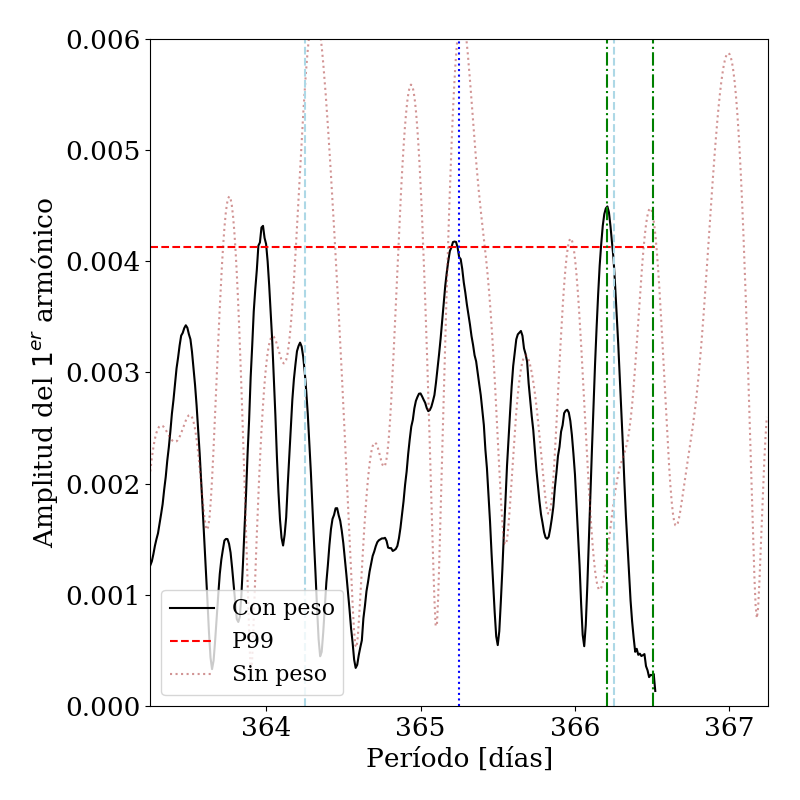
\includegraphics[width=0.5\linewidth]{zoom_anis.png}
	\caption{Zoom en el pico de anisotropía cercana para la frecuencia sidérea para el intervalo 2014-2020}
	\label{fig:zoom}
\end{figure}



\begin{table}[H]
\centering
\begin{tabular}{l|c|c|c|c}
				& Con Peso 		& Sin peso 		& Con Peso 		& Sin peso 		\\ \hline
Frecuencia:		& 366.21 		& 366.21 		& $\sim$366.505 & 366.506 		\\
Fase:			& 151.032 		& 121.695		& $\sim$190 	& 73.8188		\\
$P_{99}$:		& 0.289882\%	& 46.9691 \% 	& $\sim$96\%	& 0.24013 \% 	\\
$r_{99}$:		& 0.00512146	& 0.0018417		& $\sim$0.0006	& 0.00520328	\\
\end{tabular}
\caption{Fase, $r_{99}$ y $P_{99}$ del análisis de anisotropía entre en 1 de Enero del 2014 y el 1 de Enero del 2020}
\label{tabla:pico}
\end{table}


\section{Ajuste a orden 0 de la variación de hexágonos y pesos}

Para verificar los valores de amplitud y fase en la frecuencia sidérea, se ajusta una función del tipo $f(x) = a\cos{(2\pi\omega x + \phi)} +c$ a la variación de los hexágonos por ángulos de ascensión recta, así como también a la variación de los pesos de los hexágonos en ascensión recta. La variación y el ajuste puede verse en las Figs.\ref{fig:pesos_ajuste} y \ref{fig:pesos_hexagonos}.

\begin{figure}[H]
	\centering
	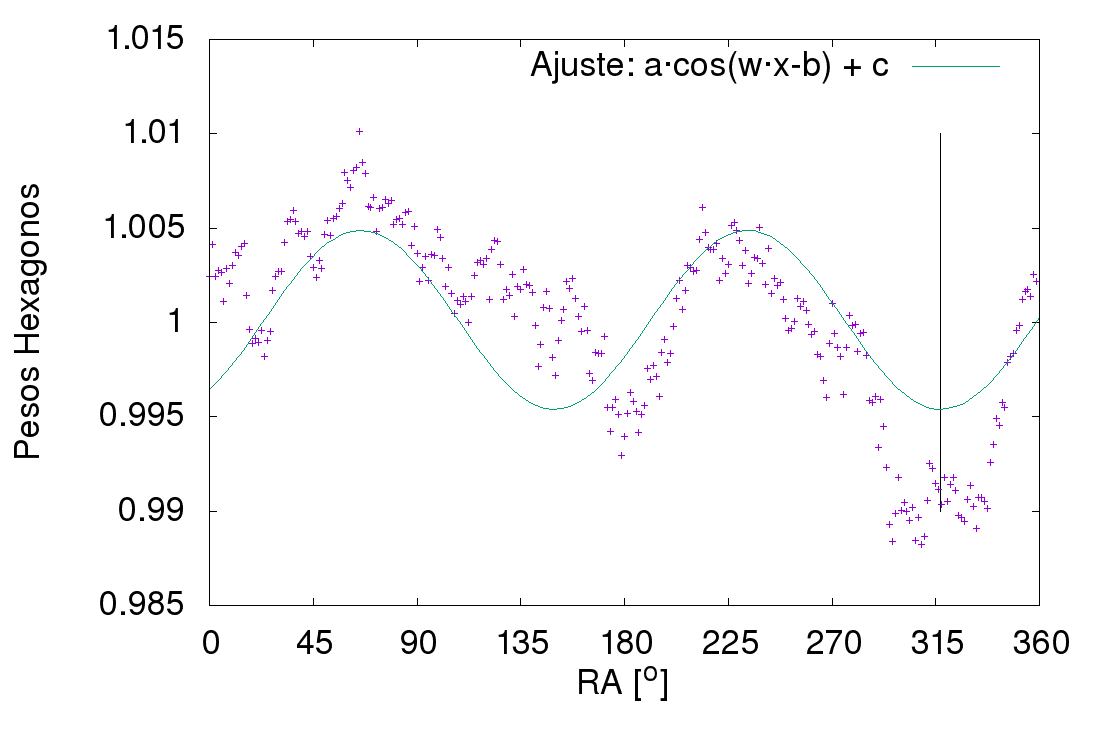
\includegraphics[width=0.5\linewidth]{ajuste_pesos.png}
	\caption{Pesos de los hexágonos para la frecuencia sidérea en el periodo 2014-2020}
	\label{fig:pesos_ajuste}
\end{figure}


\begin{figure}[H]
	\centering
	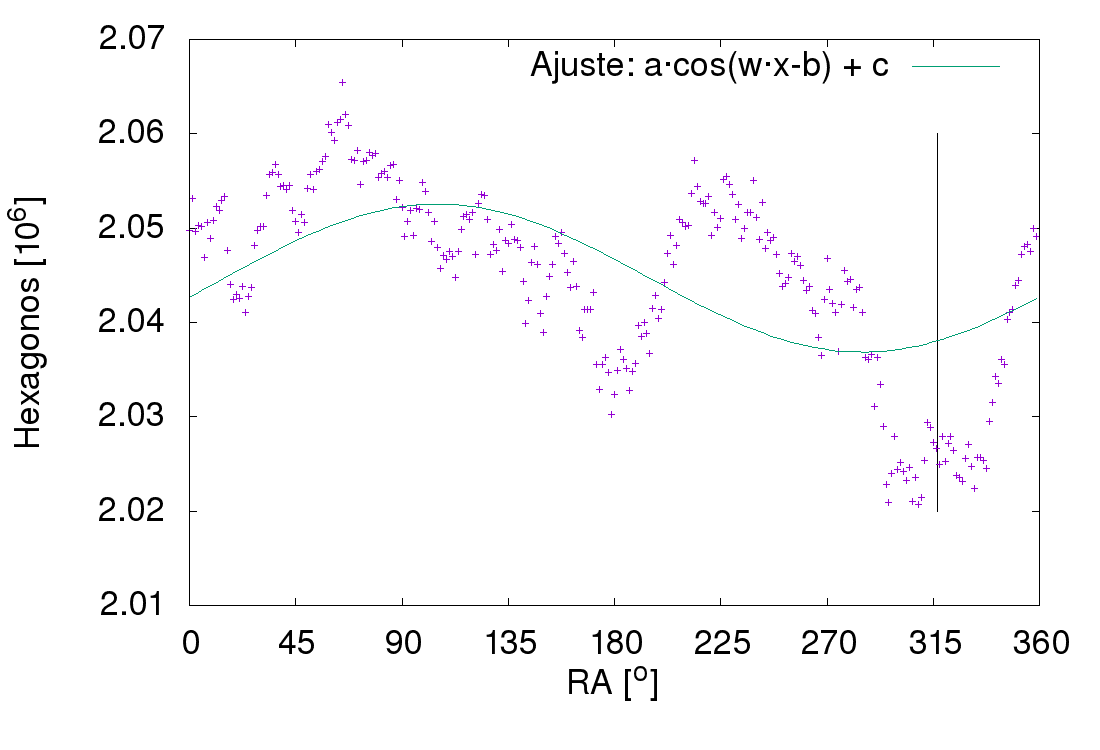
\includegraphics[width=0.5\linewidth]{ajuste_hexagonos.png}
	\caption{Hexágonos para la frecuencia sidérea en el periodo 2014-2020}
	\label{fig:pesos_hexagonos}
\end{figure}


Los valores de los ajustes, comparados con el análisis de Rayleigh se muestran en la Tabla\,\ref{tabla:ajuste_orden_cero}. SE observa que el valor de la amplitud para el caso de la variación de los pesos es más cercana al que se obtuvo en el análisis de Rayleigh. Esto puede deberse que los pesos están normalizados por la integral de todos los hexágonos dada un frecuencia, por lo que si existe alguna constante multiplicativa en la cantidad de hexágonos, la amplitud la tabla para la primera columna puede no ser igual a la segunda columna.

\begin{table}[H]
\centering
\begin{tabular}{l|c|c|c}
				& Hexágonos 				& Pesos						& Con peso \\ \hline
Figura:			& \ref{fig:pesos_hexagonos} &\ref{fig:pesos_ajuste}		&\ref{fig:zoom} \\
Fase(Mínimo):	& $\sim 317$ 				& $\sim 317$				&329.865	\\
Amplitud:		& 0.00969282 				& 0.0047421 				&0.004676\\
\end{tabular}
\caption{Fase y amplitud del ajuste a primer orden en los hexágonos y  pesos para la frecuencia sidérea}
\label{tabla:ajuste_orden_cero}
\end{table}


\end{document}